\documentclass[11pt,a4paper]{article}

% ---------------------------------------------------------------------------
% Encoding and typography
% ---------------------------------------------------------------------------

\usepackage[T1]{fontenc}
\usepackage[utf8]{inputenc}
\usepackage{lmodern}
\usepackage{microtype}

% ---------------------------------------------------------------------------
% Page layout
% ---------------------------------------------------------------------------

\usepackage[
    margin=2.5cm
]{geometry}

\usepackage{setspace}
\onehalfspacing

% ---------------------------------------------------------------------------
% Mathematics
% ---------------------------------------------------------------------------

\usepackage{amsmath}
\usepackage{amssymb}
\usepackage{mathtools}

% ---------------------------------------------------------------------------
% Units
% ---------------------------------------------------------------------------

\usepackage{siunitx}

\sisetup{
    per-mode = symbol,
    separate-uncertainty = true
}

% ---------------------------------------------------------------------------
% Tables and figures
% ---------------------------------------------------------------------------

\usepackage{graphicx}
\usepackage{booktabs}
\usepackage{array}
\usepackage{longtable}

\graphicspath{{figures/}}

% ---------------------------------------------------------------------------
% Lists
% ---------------------------------------------------------------------------

\usepackage{enumitem}

% ---------------------------------------------------------------------------
% Colors and links
% ---------------------------------------------------------------------------

\usepackage{xcolor}

\usepackage[
    colorlinks=true,
    linkcolor=blue,
    citecolor=blue,
    urlcolor=blue
]{hyperref}

\usepackage[nameinlink,noabbrev]{cleveref}


% ---------------------------------------------------------------------------
% tikz
% ---------------------------------------------------------------------------


\usepackage{tikz}
\usetikzlibrary{
    arrows.meta,
    positioning,
    shapes.geometric,
    calc
}

% ---------------------------------------------------------------------------
% Bibliography
% ---------------------------------------------------------------------------

\usepackage[
    backend=biber,
    style=numeric-comp,
    sorting=none,
    maxbibnames=99
]{biblatex}

\addbibresource{../references.bib}

% ---------------------------------------------------------------------------
% Document metadata
% ---------------------------------------------------------------------------

\title{
    \textbf{LiionTR}\\[0.5em]
    A Modular Scientific Framework for Lithium-Ion Battery Thermal Runaway Modeling
}

\author{François Dion}

\date{\today}

% ---------------------------------------------------------------------------
% Document
% ---------------------------------------------------------------------------

\begin{document}

\maketitle

\begin{abstract}

LiionTR is a modular scientific Python framework for the simulation of
lithium-ion battery thermal runaway. The framework separates thermal
runaway reaction kinetics, heat generation, gas generation, internal
pressure, venting, and numerical integration into independent physical
components.

The present formulation uses a lumped thermal model coupled to a network
of reduced-order thermal runaway reactions. Gas generation, ideal-gas
pressurization, and compressible vent flow can be incorporated into the
same numerical problem. The architecture is designed to support future
integration with thermochemical equilibrium calculations through Cantera
and electrochemical models through PyBaMM.

This report describes the mathematical formulation, software
architecture, implemented thermal runaway models, numerical methods,
verification strategy, current limitations, and planned extensions of
LiionTR.

\end{abstract}

\tableofcontents

\newpage

\section*{Nomenclature}
\addcontentsline{toc}{section}{Nomenclature}

\renewcommand{\arraystretch}{1.15}

\begin{longtable}{
    >{$}l<{$}
    p{8.3cm}
    l
}
    \toprule
    \text{Symbol} & \text{Description} & \text{Unit} \\
    \midrule
    \endfirsthead

    \toprule
    \text{Symbol} & \text{Description} & \text{Unit} \\
    \midrule
    \endhead

    A
    & Arrhenius pre-exponential factor
    & \si{\per\second}
    \\

    A_v
    & Effective vent flow area
    & \si{\meter\squared}
    \\

    A_{\mathrm{cell}}
    & External cell surface area
    & \si{\meter\squared}
    \\

    C_d
    & Vent discharge coefficient
    & --
    \\

    C_{\mathrm{th}}
    & Effective cell thermal capacity
    & \si{\joule\per\kelvin}
    \\

    c_p
    & Specific heat capacity
    & \si{\joule\per\kilogram\per\kelvin}
    \\

    c_v
    & Constant-volume specific heat capacity
    & \si{\joule\per\kilogram\per\kelvin}
    \\

    E_a
    & Activation energy
    & \si{\joule\per\mole}
    \\

    f
    & Reaction-progress function
    & --
    \\

    h
    & Convective heat-transfer coefficient
    & \si{\watt\per\meter\squared\per\kelvin}
    \\

    k(T)
    & Temperature-dependent kinetic rate coefficient
    & \si{\per\second}
    \\

    k
    & Effective thermal conductivity
    & \si{\watt\per\meter\per\kelvin}
    \\

    L_c
    & Characteristic thermal length
    & \si{\meter}
    \\

    m_{\mathrm{cell}}
    & Battery-cell mass
    & \si{\kilogram}
    \\

    m_{\mathrm{gas}}
    & Total gas mass
    & \si{\kilogram}
    \\

    \dot{m}_{\mathrm{vent}}
    & Vent mass-flow rate
    & \si{\kilogram\per\second}
    \\

    M_s
    & Molar mass of gas species $s$
    & \si{\kilogram\per\mole}
    \\

    \overline{M}
    & Mean molar mass of the gas mixture
    & \si{\kilogram\per\mole}
    \\

    n_s
    & Mole inventory of gas species $s$
    & \si{\mole}
    \\

    n_{\mathrm{tot}}
    & Total gas mole inventory
    & \si{\mole}
    \\

    \dot{n}_{s,\mathrm{gen}}
    & Generation rate of gas species $s$
    & \si{\mole\per\second}
    \\

    \dot{n}_{s,\mathrm{vent}}
    & Vent rate of gas species $s$
    & \si{\mole\per\second}
    \\

    P
    & Absolute internal gas pressure
    & \si{\pascal}
    \\

    P_0
    & Initial pressure
    & \si{\pascal}
    \\

    P_d
    & Downstream pressure
    & \si{\pascal}
    \\

    P_u
    & Upstream pressure
    & \si{\pascal}
    \\

    P_{\mathrm{vent}}
    & Vent-opening pressure
    & \si{\pascal}
    \\

    P_{\max}
    & Maximum permitted pressure
    & \si{\pascal}
    \\

    \dot{Q}_{\mathrm{gen}}
    & Total internal heat-generation rate
    & \si{\watt}
    \\

    \dot{Q}_{\mathrm{loss}}
    & Heat-loss rate
    & \si{\watt}
    \\

    \dot{q}
    & Mass-specific heat-generation rate
    & \si{\watt\per\kilogram}
    \\

    R
    & Universal gas constant
    & \si{\joule\per\mole\per\kelvin}
    \\

    R_s
    & Specific gas constant
    & \si{\joule\per\kilogram\per\kelvin}
    \\

    r
    & Remaining reaction fraction, $1-\alpha$
    & --
    \\

    r_p
    & Downstream-to-upstream pressure ratio
    & --
    \\

    r_{\mathrm{crit}}
    & Critical pressure ratio for choked flow
    & --
    \\

    T
    & Lumped cell temperature
    & \si{\kelvin}
    \\

    T_0
    & Initial cell temperature
    & \si{\kelvin}
    \\

    T_{\infty}
    & Ambient temperature
    & \si{\kelvin}
    \\

    T_{\mathrm{th}}
    & Reaction threshold temperature
    & \si{\kelvin}
    \\

    T_{\max}
    & Maximum permitted temperature
    & \si{\kelvin}
    \\

    V
    & Cell volume
    & \si{\meter\cubed}
    \\

    V_{\mathrm{free}}
    & Internal free gas volume
    & \si{\meter\cubed}
    \\

    W_i
    & Volumetric reacting-material content of reaction $i$
    & \si{\kilogram\per\meter\cubed}
    \\

    w_i
    & Effective cell mass fraction associated with reaction $i$
    & --
    \\

    x_s
    & Mole fraction of gas species $s$
    & --
    \\

    Y_{i,s}
    & Yield of gas species $s$ from reaction $i$
    & \si{\mole\per\kilogram}
    \\

    \alpha_i
    & Conversion of thermal runaway reaction $i$
    & --
    \\

    \alpha_{i,0}
    & Initial conversion of reaction $i$
    & --
    \\

    \gamma
    & Gas heat-capacity ratio, $c_p/c_v$
    & --
    \\

    \Delta H_i
    & Effective specific heat release of reaction $i$
    & \si{\joule\per\kilogram}
    \\

    \rho
    & Effective cell density
    & \si{\kilogram\per\meter\cubed}
    \\

    \boldsymbol{\alpha}
    & Vector of reaction conversions
    & --
    \\

    \mathbf{n}
    & Vector of gas-species mole inventories
    & \si{\mole}
    \\

    \mathbf{y}
    & Numerical state vector
    & --
    \\

    \mathrm{Bi}
    & Biot number
    & --
    \\

    \bottomrule
\end{longtable}

\renewcommand{\arraystretch}{1}

\newpage

\section{Introduction}
\label{sec:introduction}
Lithium-ion batteries are used extensively in transportation, portable
electronics, aerospace systems, stationary energy storage, and numerous
other applications requiring high energy density and rechargeable
electrochemical storage.

Despite their advantages, lithium-ion cells can undergo thermal runaway
when subjected to sufficiently severe thermal, electrical, mechanical,
or internal abuse conditions. Thermal runaway is characterized by a
self-accelerating sequence of exothermic reactions that can produce rapid
temperature increase, gas generation, internal pressurization, venting,
fire, and, under some conditions, propagation to neighbouring cells.

The physical processes involved span several strongly coupled domains,
including

\begin{itemize}
    \item electrochemical state evolution;
    \item decomposition reaction kinetics;
    \item heat generation and heat transfer;
    \item gas production;
    \item thermochemical gas-phase reactions;
    \item internal pressure evolution;
    \item venting and structural failure;
    \item external combustion;
    \item cell-to-cell thermal propagation.
\end{itemize}

A single mathematical model rarely represents all of these phenomena
with the same level of fidelity. Thermal runaway simulations therefore
often rely on reduced-order models calibrated against calorimetric,
abuse-test, or literature data.

LiionTR is being developed as a modular scientific framework for
constructing and solving such models while preserving a clear separation
between individual physical mechanisms.


\subsection{Project objectives}

The primary objective of LiionTR is to provide a reusable computational
framework for lithium-ion battery thermal runaway research.

The framework is designed to support:

\begin{itemize}
    \item multiple thermal runaway reaction mechanisms;
    \item reusable kinetic and reaction-progress laws;
    \item configurable battery-cell geometries and materials;
    \item thermal energy balances;
    \item empirical and future thermochemical gas-generation models;
    \item internal gas-pressure calculations;
    \item compressible venting;
    \item numerical event handling;
    \item model verification and validation;
    \item future cell-to-cell propagation models.
\end{itemize}


\subsection{Design philosophy}

A central design principle is the separation of physical models from
numerical integration.

For example, an Arrhenius model defines a temperature-dependent kinetic
rate but does not know how the corresponding reaction state is
integrated.

Similarly, a pressure model evaluates pressure from thermodynamic state
variables but does not advance those variables in time.

The numerical solver acts as the orchestration layer that assembles these
individual components into the complete governing system.

This separation is intended to improve

\begin{itemize}
    \item physical transparency;
    \item software maintainability;
    \item testability;
    \item reuse of scientific models;
    \item comparison between alternative formulations.
\end{itemize}


\subsection{Reduced-order modeling}

The current LiionTR formulation is primarily zero-dimensional.

A battery cell is represented using a lumped temperature state and a set
of scalar reaction-progress variables.

The thermal runaway process is described conceptually by

\begin{equation}
    \text{temperature}
    \rightarrow
    \text{reaction rates}
    \rightarrow
    \text{heat generation}
    \rightarrow
    \text{temperature},
\end{equation}

forming the fundamental positive feedback loop responsible for thermal
runaway.

Additional coupling can be introduced through

\begin{equation}
    \text{reaction progress}
    \rightarrow
    \text{gas generation}
    \rightarrow
    \text{pressure}
    \rightarrow
    \text{venting}.
\end{equation}

These reduced-order models are computationally inexpensive compared with
fully spatial electrochemical, thermal, mechanical, or computational
fluid dynamics models. They are therefore useful for parameter studies,
model development, sensitivity analysis, and safety-oriented system
simulations.


\subsection{Current implementation}

The present framework includes:

\begin{itemize}
    \item generic cell, geometry, and material representations;
    \item Arrhenius and threshold kinetic models;
    \item multiple reaction-progress formulations;
    \item context-dependent reaction coupling;
    \item standard and multi-channel reactions;
    \item reaction networks;
    \item a lumped thermal model;
    \item empirical reaction-based gas generation;
    \item species-resolved gas inventories;
    \item an ideal-gas pressure model;
    \item choked and unchoked compressible vent flow;
    \item irreversible vent-opening events;
    \item stiff numerical integration.
\end{itemize}

The framework also includes an implementation of the reduced-order
thermal runaway reaction model reported by
\textcite{hu2020inhibition}.


\subsection{Relationship to external scientific software}

LiionTR is not intended to reproduce capabilities that are already
provided by specialized scientific software.

Instead, external scientific packages may eventually be incorporated as
backends.

Two particularly relevant examples are Cantera and PyBaMM.

Cantera provides thermodynamic, chemical-kinetic, and transport
capabilities and is a candidate backend for equilibrium gas composition
and temperature-dependent mixture properties
\parencite{cantera2025}.

PyBaMM provides a framework for physics-based battery modeling and may
supply electrochemical states ranging from reduced-order models to
porous-electrode formulations
\parencite{sulzer2021pybamm}.

The intended long-term relationship is therefore

\begin{equation}
    \text{PyBaMM}
    \rightarrow
    \text{electrochemical state},
\end{equation}

\begin{equation}
    \text{Cantera}
    \rightarrow
    \text{thermochemical state},
\end{equation}

and

\begin{equation}
    \text{LiionTR}
    \rightarrow
    \text{thermal runaway and safety coupling}.
\end{equation}


\subsection{Scope of this report}

This report documents the mathematical formulation and current software
architecture of LiionTR.

The following sections describe:

\begin{enumerate}
    \item the general physical and mathematical framework;
    \item the lumped thermal formulation;
    \item reaction kinetics and progress models;
    \item reaction-network construction;
    \item implementation of the Hu et al.\ thermal runaway model;
    \item gas generation;
    \item pressure and venting;
    \item numerical integration;
    \item verification strategy;
    \item planned future development.
\end{enumerate}

The report describes the current state of the framework and therefore
distinguishes between implemented capabilities and planned future
extensions.

\section{Physical and Mathematical Framework}
\label{sec:framework}
LiionTR is organized around a modular formulation in which physical
models are separated from numerical integration. The objective is to
represent lithium-ion battery thermal runaway using a set of independent
but coupled subsystems describing reaction kinetics, heat generation,
gas generation, pressure evolution, and venting.

The state of a zero-dimensional LiionTR simulation can be written
conceptually as

\begin{equation}
    \mathbf{y}
    =
    \left[
        T,
        \alpha_1,
        \ldots,
        \alpha_N,
        n_1,
        \ldots,
        n_M
    \right]^{\mathrm{T}},
\end{equation}

where $T$ is the lumped cell temperature, $\alpha_i$ is the conversion
of thermal runaway reaction $i$, and $n_s$ is the amount of gas species
$s$ contained in the cell free volume.

The governing system may therefore be expressed as

\begin{equation}
    \frac{d\mathbf{y}}{dt}
    =
    \mathbf{F}
    \left(
        t,
        \mathbf{y}
    \right),
\end{equation}

where the right-hand side is assembled from the thermal, reaction,
gas-generation, pressure, and vent-flow models.


\subsection{Thermal state}

The cell temperature evolves according to an energy balance,

\begin{equation}
    C_{\mathrm{th}}
    \frac{dT}{dt}
    =
    \dot{Q}_{\mathrm{gen}}
    -
    \dot{Q}_{\mathrm{loss}},
    \label{eq:general_energy_balance}
\end{equation}

where $C_{\mathrm{th}}$ is the effective cell thermal capacity,
$\dot{Q}_{\mathrm{gen}}$ is the total internal heat-generation rate, and
$\dot{Q}_{\mathrm{loss}}$ is the heat-transfer rate from the cell to its
environment.


\subsection{Reaction states}

Each thermal runaway reaction is represented using a scalar conversion,

\begin{equation}
    0
    \leq
    \alpha_i
    \leq
    1.
\end{equation}

The corresponding reaction rate is represented by

\begin{equation}
    \frac{d\alpha_i}{dt}
    =
    k_i(T)
    f_i
    \left(
        \alpha_i,
        \mathbf{\alpha}
    \right),
    \label{eq:reaction_progress_general}
\end{equation}

where $k_i(T)$ describes the intrinsic temperature dependence and
$f_i$ describes the dependence on reaction progress and, when required,
the state of other reactions.

The complete reaction-state vector is

\begin{equation}
    \boldsymbol{\alpha}
    =
    \left[
        \alpha_1,
        \alpha_2,
        \ldots,
        \alpha_N
    \right]^{\mathrm{T}}.
\end{equation}


\subsection{Heat generation}

For a reaction occupying an effective cell mass fraction $w_i$ and
releasing a specific enthalpy $\Delta H_i$, the mass-specific
heat-generation rate is written as

\begin{equation}
    \dot{q}_i
    =
    w_i
    \Delta H_i
    \frac{d\alpha_i}{dt}.
\end{equation}

The total heat-generation rate for a cell of mass $m_{\mathrm{cell}}$
is then

\begin{equation}
    \dot{Q}_{\mathrm{gen}}
    =
    m_{\mathrm{cell}}
    \sum_{i=1}^{N}
    \dot{q}_i.
    \label{eq:total_heat_generation}
\end{equation}


\subsection{Gas-generation states}

When gas generation is enabled, each gas species is represented by a
mole inventory $n_s$.

Before vent opening,

\begin{equation}
    \frac{dn_s}{dt}
    =
    \dot{n}_{s,\mathrm{gen}},
\end{equation}

where $\dot{n}_{s,\mathrm{gen}}$ is the molar gas-generation rate.

After vent opening,

\begin{equation}
    \frac{dn_s}{dt}
    =
    \dot{n}_{s,\mathrm{gen}}
    -
    \dot{n}_{s,\mathrm{vent}}.
    \label{eq:vented_species_balance}
\end{equation}


\subsection{Pressure state}

The current reduced-order formulation evaluates internal gas pressure
using the ideal-gas equation,

\begin{equation}
    P
    =
    \frac{
        n_{\mathrm{tot}} R T
    }{
        V_{\mathrm{free}}
    },
    \label{eq:ideal_pressure_framework}
\end{equation}

where

\begin{equation}
    n_{\mathrm{tot}}
    =
    \sum_{s=1}^{M}
    n_s.
\end{equation}

The current formulation assumes that the gas temperature is equal to the
lumped cell temperature.


\subsection{Model coupling}

The principal physical couplings represented in LiionTR are

\begin{enumerate}
    \item temperature controls thermal runaway reaction rates;
    \item thermal runaway reactions release heat;
    \item heat generation modifies the cell temperature;
    \item reaction progress can generate gas;
    \item the gas inventory and temperature determine internal pressure;
    \item internal pressure can trigger vent opening;
    \item vent flow removes gas from the internal inventory.
\end{enumerate}

The reaction-thermal coupling forms the fundamental positive feedback
mechanism responsible for thermal runaway.

A conceptual representation of the current LiionTR architecture is shown
in Figure~\ref{fig:framework_architecture}.

\begin{figure}[htbp]
    \centering
    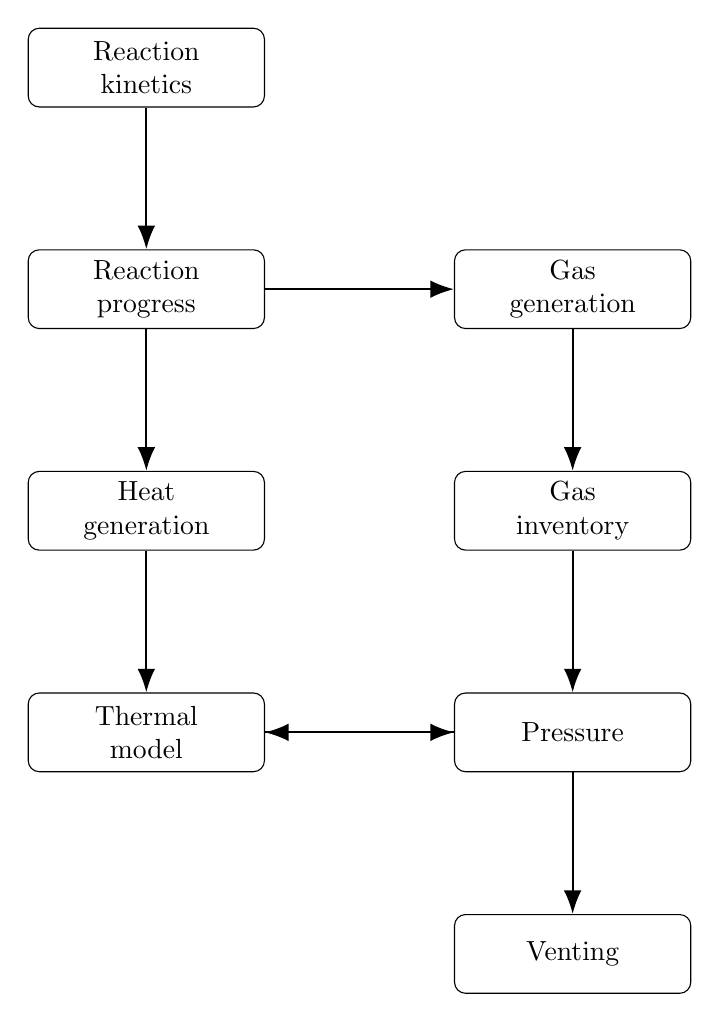
\begin{tikzpicture}[
        node distance=1.8cm and 2.4cm,
        block/.style={
            rectangle,
            rounded corners,
            draw,
            align=center,
            minimum width=3.0cm,
            minimum height=1.0cm
        },
        line/.style={
            -{Latex[length=3mm]},
            thick
        }
    ]

    \node[block] (kinetics) {Reaction\\kinetics};
    \node[block, below=of kinetics] (progress) {Reaction\\progress};
    \node[block, below=of progress] (heat) {Heat\\generation};
    \node[block, below=of heat] (thermal) {Thermal\\model};

    \node[block, right=of progress] (gasgen) {Gas\\generation};
    \node[block, below=of gasgen] (inventory) {Gas\\inventory};
    \node[block, below=of inventory] (pressure) {Pressure};
    \node[block, below=of pressure] (venting) {Venting};

    \draw[line] (kinetics) -- (progress);
    \draw[line] (progress) -- (heat);
    \draw[line] (heat) -- (thermal);

    \draw[line] (progress) -- (gasgen);
    \draw[line] (gasgen) -- (inventory);
    \draw[line] (inventory) -- (pressure);
    \draw[line] (pressure) -- (venting);

    \draw[line] (thermal.east) -- ++(1.2,0) |- (pressure.west);
    \draw[line] (pressure.west) -- ++(-1.2,0) |- (thermal.east);

    \end{tikzpicture}
    \caption{
        Conceptual architecture of the current LiionTR framework.
        Reaction kinetics determine reaction progress, which drives both
        heat generation and gas generation. Heat generation affects the
        thermal model, while gas generation affects the gas inventory and
        therefore the internal pressure. Pressure may eventually trigger
        venting.
    }
    \label{fig:framework_architecture}
\end{figure}


\subsection{Separation of physical models and state integration}

A central design principle of LiionTR is that physical model objects do
not advance their own numerical state.

Instead, the numerical solver owns the complete state vector and passes
the current state to the physical models whenever the right-hand side is
evaluated.

This design provides several advantages:

\begin{itemize}
    \item deterministic evaluation of the governing equations;
    \item compatibility with standard ordinary differential equation
          solvers;
    \item reduced hidden coupling between physical components;
    \item independent verification of individual physical models;
    \item easier implementation of event handling and future alternative
          numerical solvers.
\end{itemize}


\subsection{Scope of the present framework}

The current implementation focuses on reduced-order, zero-dimensional
thermal runaway modeling.

The framework is intended to evolve toward more comprehensive physical
descriptions, including thermochemical equilibrium, detailed
electrochemical state information, spatially resolved heat transfer,
cell-to-cell propagation, structural failure, and external vent-jet or
combustion models.

Cantera is considered as a future thermochemical backend, while PyBaMM
may provide electrochemical states and normal-operation battery physics.
LiionTR is intended to remain the orchestration layer responsible for
thermal runaway and battery-safety-specific coupling.

\section{Thermal Model}
\label{sec:thermal}
The current LiionTR thermal formulation uses a zero-dimensional
lumped-capacitance model. The complete battery cell is represented by a
single temperature state, such that internal spatial temperature
gradients are neglected.

The thermal energy balance is

\begin{equation}
    C_{\mathrm{th}}
    \frac{dT}{dt}
    =
    \dot{Q}_{\mathrm{gen}}
    -
    h A
    \left(
        T - T_{\infty}
    \right),
    \label{eq:lumped_thermal_balance}
\end{equation}

where $C_{\mathrm{th}}$ is the cell thermal capacity,
$\dot{Q}_{\mathrm{gen}}$ is the total internal heat-generation rate,
$h$ is the convective heat-transfer coefficient, $A$ is the external
cell surface area, and $T_{\infty}$ is the ambient temperature.

The resulting temperature derivative is

\begin{equation}
    \frac{dT}{dt}
    =
    \frac{
        \dot{Q}_{\mathrm{gen}}
        -
        h A
        \left(
            T-T_{\infty}
        \right)
    }{
        C_{\mathrm{th}}
    }.
    \label{eq:lumped_temperature_derivative}
\end{equation}


\subsection{Cell thermal capacity}

The effective thermal capacity is calculated as

\begin{equation}
    C_{\mathrm{th}}
    =
    m_{\mathrm{cell}}
    c_p,
    \label{eq:thermal_capacity}
\end{equation}

where $c_p$ is the effective specific heat capacity of the cell.

The cell mass is calculated from the effective density and geometry,

\begin{equation}
    m_{\mathrm{cell}}
    =
    \rho V,
    \label{eq:cell_mass}
\end{equation}

leading to

\begin{equation}
    C_{\mathrm{th}}
    =
    \rho V c_p.
\end{equation}

In the present implementation, density and specific heat capacity are
evaluated at \SI{298.15}{\kelvin} when cell mass and thermal capacity
are constructed. These quantities are therefore constant during a
simulation.


\subsection{Convective heat transfer}

Heat exchange with the environment is currently represented using
Newton's law of cooling,

\begin{equation}
    \dot{Q}_{\mathrm{conv}}
    =
    h A
    \left(
        T - T_{\infty}
    \right).
    \label{eq:convective_heat_loss}
\end{equation}

When $T>T_{\infty}$, this term removes heat from the cell.

If $T<T_{\infty}$, the same expression becomes negative and therefore
represents heating of the cell by the surrounding environment.


\subsection{Internal heat generation}

Internal heat generation is supplied to the thermal model by the
configured chemistry backend.

For a reaction network containing $N$ thermal runaway reactions,

\begin{equation}
    \dot{Q}_{\mathrm{gen}}
    =
    m_{\mathrm{cell}}
    \sum_{i=1}^{N}
    w_i
    \Delta H_i
    \dot{\alpha}_i.
    \label{eq:thermal_reaction_heat}
\end{equation}

The thermal model is therefore independent from the detailed kinetic
mechanism. Different reaction networks can be coupled to the same
thermal formulation.


\subsection{Thermal runaway feedback}

The coupling between reaction kinetics and temperature introduces a
positive feedback mechanism.

For Arrhenius kinetics,

\begin{equation}
    k(T)
    =
    A
    \exp
    \left(
        -\frac{E_a}{RT}
    \right).
\end{equation}

As temperature rises, the reaction rate generally increases. This
increases heat generation, which produces further temperature increase.

Conceptually,

\begin{equation}
    T
    \uparrow
    \quad \Longrightarrow \quad
    k(T)
    \uparrow
    \quad \Longrightarrow \quad
    \dot{Q}_{\mathrm{gen}}
    \uparrow
    \quad \Longrightarrow \quad
    T
    \uparrow.
\end{equation}

This feedback constitutes the principal mechanism of thermal runaway in
the present reduced-order framework.


\subsection{Validity of the lumped approximation}

The lumped-capacitance approximation assumes that the internal
temperature field equilibrates sufficiently rapidly compared with heat
transfer across the external boundary.

A conventional criterion is the Biot number,

\begin{equation}
    \mathrm{Bi}
    =
    \frac{
        h L_c
    }{
        k
    },
\end{equation}

where $L_c$ is a characteristic cell length and $k$ is the effective
thermal conductivity.

The lumped approximation is generally most appropriate when

\begin{equation}
    \mathrm{Bi}
    \ll
    1.
\end{equation}

LiionTR does not currently enforce a Biot-number criterion. Consequently,
the validity of the lumped approximation must be assessed for the
geometry, boundary conditions, and thermal runaway regime being
simulated.


\subsection{Current assumptions}

The present thermal formulation assumes:

\begin{itemize}
    \item a spatially uniform cell temperature;
    \item constant effective thermophysical properties;
    \item constant ambient temperature;
    \item uniform convection over the complete external cell surface;
    \item no radiative heat transfer;
    \item no explicit conductive coupling to neighbouring cells or
          structures;
    \item no explicit phase-change enthalpy;
    \item no internal thermal gradients.
\end{itemize}


\subsection{Limitations and future extensions}

A single-temperature model cannot reproduce internal hot spots or
temperature gradients that may develop during severe thermal runaway.

Future thermal-model developments may therefore include:

\begin{itemize}
    \item temperature-dependent density, heat capacity, and thermal
          conductivity;
    \item radiative heat transfer;
    \item conductive coupling between cells;
    \item one-dimensional or multidimensional thermal models;
    \item cell-to-cell thermal propagation;
    \item latent-heat and phase-change effects;
    \item energy coupling to vented material and gas enthalpy.
\end{itemize}

\section{Reaction Kinetics}
\label{sec:kinetics}
Thermal runaway reactions are represented using reduced-order kinetic
models that relate reaction progress to temperature and reaction state.

For reaction $i$, the general progress equation is

\begin{equation}
    \frac{d\alpha_i}{dt}
    =
    k_i(T)
    f_i
    \left(
        \alpha_i,
        \mathbf{\alpha}
    \right),
    \label{eq:general_kinetics}
\end{equation}

where $\alpha_i$ is the dimensionless reaction conversion,
$k_i(T)$ is the intrinsic temperature-dependent rate coefficient, and
$f_i$ is a progress function that may depend on the state of the
complete reaction network.


\subsection{Reaction conversion}

Reaction progress is represented by a conversion variable satisfying

\begin{equation}
    0
    \leq
    \alpha
    \leq
    1.
\end{equation}

The unreacted or remaining fraction is therefore

\begin{equation}
    r
    =
    1-\alpha.
\end{equation}

An unreacted state corresponds to $\alpha=0$, while a fully reacted
state corresponds to $\alpha=1$.


\subsection{Arrhenius kinetics}

The principal kinetic model currently implemented in LiionTR is the
Arrhenius relation,

\begin{equation}
    k(T)
    =
    A
    \exp
    \left(
        -\frac{E_a}{RT}
    \right),
    \label{eq:arrhenius}
\end{equation}

where $A$ is the pre-exponential factor, $E_a$ is the activation energy,
$R$ is the universal gas constant, and $T$ is the absolute temperature.

For first-order kinetics, $A$ has units of \si{\per\second}, while
$E_a$ is expressed in \si{\joule\per\mole}.

The exponential temperature dependence is central to thermal runaway.
A relatively modest increase in temperature can produce a large increase
in reaction rate, thereby increasing heat generation and further
accelerating the thermal response.


\subsection{Power-law progress}

A common progress model is based on the remaining reactant fraction,

\begin{equation}
    f(\alpha)
    =
    \left(
        1-\alpha
    \right)^n,
    \label{eq:power_law_progress}
\end{equation}

where $n$ is the reaction order.

The complete progress equation becomes

\begin{equation}
    \frac{d\alpha}{dt}
    =
    A
    \exp
    \left(
        -\frac{E_a}{RT}
    \right)
    \left(
        1-\alpha
    \right)^n.
\end{equation}

For $n=1$, the reaction rate decreases linearly with the remaining
reactant fraction.


\subsection{Autocatalytic progress}

LiionTR also supports autocatalytic progress laws of the general form

\begin{equation}
    f(\alpha)
    =
    \alpha^m
    \left(
        1-\alpha
    \right)^n,
    \label{eq:autocatalytic_progress}
\end{equation}

where $m$ and $n$ control the dependence on reacted and unreacted
material, respectively.

Such a formulation can represent reactions that accelerate as reaction
products or active sites accumulate before eventually slowing as the
reactant is depleted.

A frequently used special case is

\begin{equation}
    f(\alpha)
    =
    \alpha
    \left(
        1-\alpha
    \right).
\end{equation}


\subsection{Temperature thresholds}

Some reduced-order models assume that a reaction is inactive below a
prescribed onset temperature.

LiionTR represents this using a thresholded kinetic rate,

\begin{equation}
    k_{\mathrm{th}}(T)
    =
    \begin{cases}
        0,
        & T < T_{\mathrm{th}},
        \\[6pt]
        k(T),
        & T \geq T_{\mathrm{th}}.
    \end{cases}
    \label{eq:temperature_threshold}
\end{equation}

This formulation is useful when reproducing empirical literature models
that prescribe an explicit reaction onset temperature.


\subsection{Context-dependent reaction progress}

Thermal runaway reactions are not always independent.

The progress of one reaction may depend on the state of another
reaction, such as the depletion of a protective layer or the formation
of reactive products.

LiionTR therefore allows a progress model to depend on a reaction
context containing the complete conversion vector,

\begin{equation}
    \boldsymbol{\alpha}
    =
    \left[
        \alpha_1,
        \alpha_2,
        \ldots,
        \alpha_N
    \right]^{\mathrm{T}}.
\end{equation}

The progress equation can therefore be written more generally as

\begin{equation}
    \frac{d\alpha_i}{dt}
    =
    k_i(T)
    f_i
    \left(
        \alpha_i,
        \boldsymbol{\alpha}
    \right).
\end{equation}


\subsection{Threshold progress}

A context-dependent reaction may be activated only when another state
variable satisfies a prescribed condition.

For a context variable $x$, a generic threshold progress model may be
written as

\begin{equation}
    f_{\mathrm{th}}
    =
    \begin{cases}
        0,
        & x > x_{\mathrm{th}},
        \\[6pt]
        f(\alpha),
        & x \leq x_{\mathrm{th}}.
    \end{cases}
    \label{eq:progress_threshold}
\end{equation}

This formulation is used to represent sequential or conditionally
activated thermal runaway mechanisms.


\subsection{Exponential inhibition}

LiionTR also provides an exponential inhibition mechanism,

\begin{equation}
    f_{\mathrm{inh}}
    =
    f(\alpha)
    \exp(-x),
    \label{eq:exponential_inhibition}
\end{equation}

where $x$ is a context-dependent inhibition variable.

As $x$ increases, the effective reaction rate decreases exponentially.

Such a formulation can represent the influence of a protective layer or
other inhibiting material on a subsequent reaction.


\subsection{Normalized context variables}

A context variable may be constructed from the conversion or remaining
fraction of another reaction.

For example, the remaining fraction of reaction $j$ is

\begin{equation}
    r_j
    =
    1-\alpha_j.
\end{equation}

A normalized remaining-fraction variable may then be defined as

\begin{equation}
    x_j
    =
    \frac{
        r_j
    }{
        r_{\mathrm{ref}}
    },
    \label{eq:normalized_remaining_fraction}
\end{equation}

where $r_{\mathrm{ref}}$ is a prescribed reference value.

This provides a flexible mechanism for reproducing coupling terms
reported in reduced-order thermal runaway models.


\subsection{Separation of kinetics and progress}

LiionTR deliberately separates the intrinsic kinetic law from the
reaction-progress model.

The kinetic model determines how temperature affects the intrinsic rate,

\begin{equation}
    T
    \longrightarrow
    k(T),
\end{equation}

while the progress model determines how reaction state modifies that
rate,

\begin{equation}
    \boldsymbol{\alpha}
    \longrightarrow
    f
    \left(
        \alpha,
        \boldsymbol{\alpha}
    \right).
\end{equation}

The complete progress rate is obtained only after combining both terms.

This separation permits a common kinetic model, such as Arrhenius
kinetics, to be reused with multiple progress laws.


\subsection{Current limitations}

The present kinetic framework is intended primarily for reduced-order
thermal runaway modeling.

Current limitations include:

\begin{itemize}
    \item no explicit pressure dependence in the standard kinetic laws;
    \item no transport-limited reaction formulation;
    \item no explicit dependence on electrode potential or lithium
          concentration;
    \item no uncertainty propagation for kinetic parameters;
    \item no automatic kinetic parameter estimation from calorimetric
          data;
    \item no automatic competition between alternative reaction
          mechanisms.
\end{itemize}

Future developments may include parameter calibration using ARC or DSC
data, uncertainty quantification, and coupling to electrochemical state
variables supplied by PyBaMM.

\section{Reaction Network}
\label{sec:reactions}
The reaction subsystem combines kinetic laws, reaction-progress models,
reaction enthalpies, and reacting-material inventories into physical
thermal runaway reactions.

Each reaction contributes both a progress rate and a heat-generation
rate to the coupled system.


\subsection{Standard reaction model}

For a standard reaction, the progress rate is

\begin{equation}
    \dot{\alpha}
    =
    k(T)
    f
    \left(
        \alpha,
        \boldsymbol{\alpha}
    \right),
    \label{eq:reaction_progress}
\end{equation}

where $k(T)$ is the kinetic rate and $f$ is the reaction-progress
function.

If the reaction occupies an effective mass fraction $w$ of the total
cell mass and releases a specific enthalpy $\Delta H$, the
mass-specific heat-generation rate relative to total cell mass is

\begin{equation}
    \dot{q}
    =
    w
    \Delta H
    \dot{\alpha}.
    \label{eq:reaction_heat_specific}
\end{equation}

The total heat-generation rate for a cell of mass $m_{\mathrm{cell}}$
is therefore

\begin{equation}
    \dot{Q}
    =
    m_{\mathrm{cell}}
    w
    \Delta H
    \dot{\alpha}.
    \label{eq:reaction_heat_total}
\end{equation}


\subsection{Reaction enthalpy convention}

The parameter $\Delta H$ represents the effective heat release per unit
mass of reacting material.

For the reduced-order exothermic reactions currently implemented,
$\Delta H$ is treated as a positive heat-release quantity.

The resulting heat-generation term is therefore positive when

\begin{equation}
    \dot{\alpha} > 0.
\end{equation}

This convention avoids embedding thermodynamic sign conventions directly
into the thermal balance and is consistent with the current LiionTR
reaction implementation.


\subsection{Reaction mass fraction}

The parameter $w$ represents the effective fraction of total cell mass
participating in a particular reaction.

For literature models that report a volumetric reactant content
$W_r$ in \si{\kilogram\per\meter\cubed}, LiionTR converts this quantity
to a cell mass fraction using

\begin{equation}
    w
    =
    \frac{
        W_r
    }{
        \rho_{\mathrm{cell}}
    },
    \label{eq:volumetric_to_mass_fraction}
\end{equation}

where $\rho_{\mathrm{cell}}$ is the effective cell density.

This conversion enables literature models reported on a volumetric basis
to be used consistently within the cell-mass-based thermal formulation.


\subsection{Reaction context}

Individual reactions may depend on the state of other reactions.

LiionTR therefore constructs a reaction context containing the complete
reaction state

\begin{equation}
    \boldsymbol{\alpha}
    =
    \left[
        \alpha_1,
        \ldots,
        \alpha_N
    \right]^{\mathrm{T}}.
\end{equation}

The context provides access to quantities such as

\begin{equation}
    \alpha_j
\end{equation}

and

\begin{equation}
    1-\alpha_j,
\end{equation}

as well as transformed or normalized context variables.

This permits reaction coupling without storing mutable integration state
inside individual reaction objects.


\subsection{Multi-channel reactions}

Some literature models represent one physical decomposition process
using several parallel kinetic channels.

LiionTR represents these processes with a common conversion variable and
multiple kinetic channels.

The shared reaction progress rate is obtained from the sum of the
individual kinetic channels,

\begin{equation}
    \dot{\alpha}
    =
    f
    \left(
        \alpha,
        \boldsymbol{\alpha}
    \right)
    \sum_{j=1}^{N_c}
    k_j(T).
    \label{eq:multichannel_progress}
\end{equation}

For $N_c$ channels sharing a conversion $\alpha$, the heat-generation
rate can be written conceptually as


\begin{equation}
    \dot{q}
    =
    w
    f
    \left(
        \alpha,
        \boldsymbol{\alpha}
    \right)
    \sum_{j=1}^{N_c}
    \Delta H_j
    k_j(T).
    \label{eq:multichannel_heat}
\end{equation}

Each channel therefore contributes independently to heat generation,
while the physical reaction retains only one integrated progress state.


\subsection{Shared reaction progress}

The use of a shared conversion is physically distinct from representing
each kinetic channel as an independent reaction.

For a multi-channel decomposition mechanism, all channels consume the
same effective reactant inventory.

The model therefore integrates

\begin{equation}
    \alpha
\end{equation}

rather than introducing separate conversions

\begin{equation}
    \alpha_1,
    \alpha_2,
    \ldots,
    \alpha_{N_c}.
\end{equation}

This distinction is important for preserving a consistent reacting mass
inventory.


\subsection{Reaction network}

A thermal runaway mechanism is assembled as a network containing
multiple reactions.

For $N$ reactions, the conversion vector is

\begin{equation}
    \boldsymbol{\alpha}
    =
    \left[
        \alpha_1,
        \alpha_2,
        \ldots,
        \alpha_N
    \right]^{\mathrm{T}}.
\end{equation}

The corresponding progress-rate vector is

\begin{equation}
    \dot{\boldsymbol{\alpha}}
    =
    \left[
        \dot{\alpha}_1,
        \dot{\alpha}_2,
        \ldots,
        \dot{\alpha}_N
    \right]^{\mathrm{T}}.
\end{equation}

Each reaction is evaluated using the current temperature and current
reaction-network state.


\subsection{Network heat generation}

The total mass-specific heat-generation rate is

\begin{equation}
    \dot{q}_{\mathrm{total}}
    =
    \sum_{i=1}^{N}
    \dot{q}_i.
    \label{eq:network_specific_heat}
\end{equation}

The corresponding total cell heat-generation rate is

\begin{equation}
    \dot{Q}_{\mathrm{gen}}
    =
    m_{\mathrm{cell}}
    \dot{q}_{\mathrm{total}}.
    \label{eq:network_total_heat}
\end{equation}

This quantity is passed to the thermal model.


\subsection{Coupled thermal-reaction system}

The reaction network and thermal model form a strongly coupled
nonlinear system,

\begin{equation}
    \frac{dT}{dt}
    =
    \frac{
        m_{\mathrm{cell}}
        \displaystyle\sum_{i=1}^{N}
        \dot{q}_i
        -
        hA
        \left(
            T-T_{\infty}
        \right)
    }{
        C_{\mathrm{th}}
    },
    \label{eq:coupled_temperature}
\end{equation}

with

\begin{equation}
    \frac{d\alpha_i}{dt}
    =
    k_i(T)
    f_i
    \left(
        \alpha_i,
        \boldsymbol{\alpha}
    \right),
    \qquad
    i=1,\ldots,N.
    \label{eq:coupled_reactions}
\end{equation}

The reaction rates depend on temperature, while temperature depends on
reaction heat generation.

This bidirectional coupling produces the positive feedback characteristic
of thermal runaway.


\subsection{Initial reaction state}

Each reaction requires an initial conversion

\begin{equation}
    \alpha_{i,0}.
\end{equation}

The complete initial reaction state is

\begin{equation}
    \boldsymbol{\alpha}_0
    =
    \left[
        \alpha_{1,0},
        \ldots,
        \alpha_{N,0}
    \right]^{\mathrm{T}}.
\end{equation}

When a literature model reports an initial remaining fraction $r_0$,
LiionTR converts it using

\begin{equation}
    \alpha_0
    =
    1-r_0.
    \label{eq:remaining_to_conversion}
\end{equation}


\subsection{Software representation}

The physical organization of the reaction subsystem can be summarized
using the conceptual structure shown in
Figure~\ref{fig:reaction_architecture}.

\begin{figure}[htbp]
    \centering

    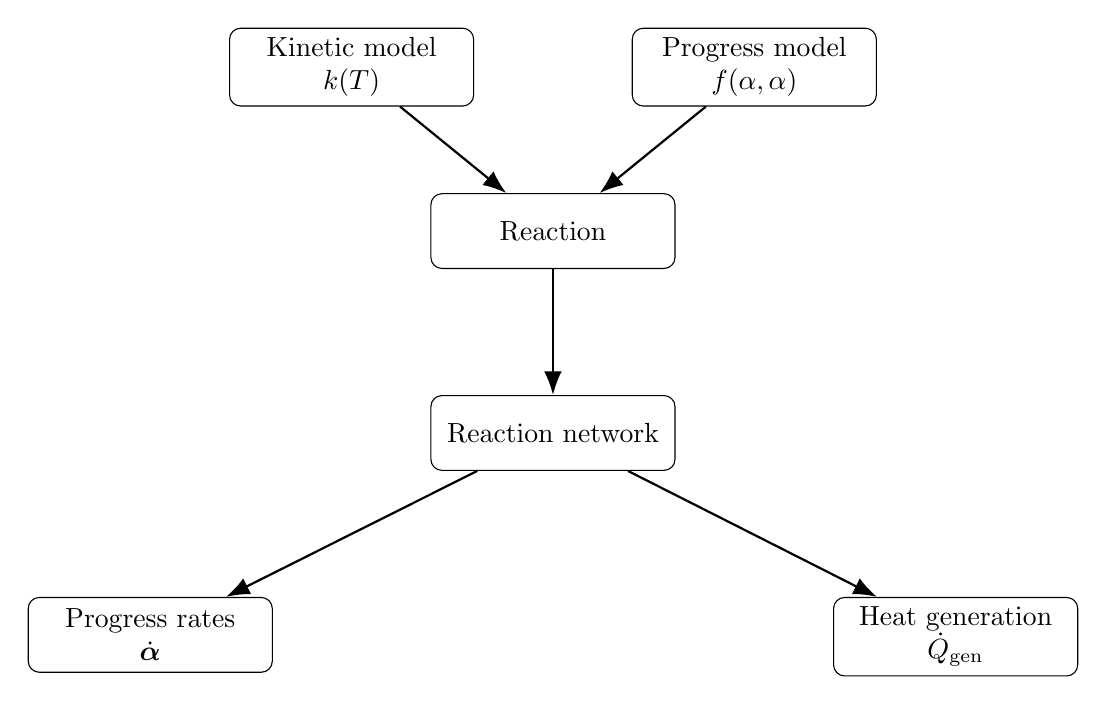
\begin{tikzpicture}[
        node distance=1.6cm and 2.0cm,
        block/.style={
            rectangle,
            rounded corners,
            draw,
            align=center,
            minimum width=3.1cm,
            minimum height=0.95cm
        },
        line/.style={
            -{Latex[length=3mm]},
            thick
        }
    ]

    \node[block] (kinetic) {Kinetic model\\$k(T)$};
    \node[block, right=of kinetic] (progress) {Progress model\\$f(\alpha,\mathbf{\alpha})$};

    \node[block, below=of $(kinetic)!0.5!(progress)$] (reaction)
        {Reaction};

    \node[block, below=of reaction] (network)
        {Reaction network};

    \node[block, below left=of network] (rates)
        {Progress rates\\$\dot{\boldsymbol{\alpha}}$};

    \node[block, below right=of network] (heat)
        {Heat generation\\$\dot{Q}_{\mathrm{gen}}$};

    \draw[line] (kinetic) -- (reaction);
    \draw[line] (progress) -- (reaction);
    \draw[line] (reaction) -- (network);
    \draw[line] (network) -- (rates);
    \draw[line] (network) -- (heat);

    \end{tikzpicture}

    \caption{
        Conceptual organization of the LiionTR reaction subsystem.
        Kinetic and progress models are combined into reaction models,
        which are assembled into a reaction network that supplies
        reaction progress rates and total heat generation.
    }
    \label{fig:reaction_architecture}
\end{figure}


\subsection{Current assumptions}

The current reaction framework assumes that:

\begin{itemize}
    \item every integrated reaction is represented by a scalar conversion;
    \item reaction states are spatially uniform;
    \item reaction enthalpies are effective constant quantities;
    \item reacting-material mass fractions remain fixed;
    \item pressure dependence is absent unless explicitly introduced by a
          custom model;
    \item reaction products are not automatically determined from
          chemical equilibrium;
    \item transport limitations are not explicitly resolved.
\end{itemize}


\subsection{Future extensions}

The modular reaction architecture is intended to support more detailed
physical descriptions.

Potential extensions include:

\begin{itemize}
    \item temperature-dependent reaction enthalpies;
    \item pressure-dependent kinetics;
    \item transport-limited reactions;
    \item competing reaction mechanisms;
    \item reaction-derived elemental source inventories;
    \item thermochemical equilibrium using Cantera;
    \item electrochemical-state-dependent kinetics;
    \item calibration against ARC and DSC measurements;
    \item parameter uncertainty and sensitivity analysis.
\end{itemize}

\section{Hu et al. (2020) Thermal Runaway Model}
\label{sec:hu2020}
The first complete thermal runaway reaction network implemented in
LiionTR is based on the reduced-order model reported by
\textcite{hu2020inhibition}.

The model represents thermal runaway using four principal reaction
states:

\begin{enumerate}
    \item solid-electrolyte interphase (SEI) decomposition;
    \item anode-electrolyte reaction;
    \item cathode decomposition;
    \item electrolyte decomposition.
\end{enumerate}

Rather than implementing the model as a single monolithic component,
LiionTR represents each physical contribution using the generic kinetic,
progress, reaction, and reaction-network abstractions described in
\cref{sec:kinetics,sec:reactions}.


\subsection{Reaction-state vector}

The reaction-state vector is

\begin{equation}
    \boldsymbol{\alpha}
    =
    \begin{bmatrix}
        \alpha_{\mathrm{SEI}} \\
        \alpha_{\mathrm{an}} \\
        \alpha_{\mathrm{cat}} \\
        \alpha_{\mathrm{el}}
    \end{bmatrix},
    \label{eq:hu_state_vector}
\end{equation}

where the subscripts denote SEI decomposition, anode-electrolyte
reaction, cathode decomposition, and electrolyte decomposition,
respectively.

The initial state used by the current LiionTR implementation is

\begin{equation}
    \boldsymbol{\alpha}_0
    =
    \begin{bmatrix}
        0.85 \\
        0.25 \\
        0.04 \\
        0.00
    \end{bmatrix}.
    \label{eq:hu_initial_state}
\end{equation}


\subsection{Arrhenius formulation}

The thermally activated reactions use the Arrhenius expression

\begin{equation}
    k_i(T)
    =
    A_i
    \exp
    \left(
        -\frac{E_{a,i}}{RT}
    \right),
    \label{eq:hu_arrhenius}
\end{equation}

where $A_i$ is the pre-exponential factor and $E_{a,i}$ is the
activation energy of reaction $i$.

The resulting conversion rate is obtained by multiplying the kinetic
term by the appropriate reaction-progress model,

\begin{equation}
    \dot{\alpha}_i
    =
    k_i(T)
    f_i
    \left(
        \alpha_i,
        \boldsymbol{\alpha}
    \right).
    \label{eq:hu_generic_progress}
\end{equation}


\subsection{SEI decomposition}

The SEI decomposition reaction is represented using first-order
remaining-fraction kinetics,

\begin{equation}
    \frac{d\alpha_{\mathrm{SEI}}}{dt}
    =
    k_{\mathrm{SEI}}(T)
    \left(
        1-\alpha_{\mathrm{SEI}}
    \right).
    \label{eq:hu_sei_progress}
\end{equation}

The implemented kinetic parameters are

\begin{align}
    A_{\mathrm{SEI}}
    &=
    \num{1.667e15}
    \ \si{\per\second},
    \\
    E_{a,\mathrm{SEI}}
    &=
    \num{1.3508e5}
    \ \si{\joule\per\mole},
    \\
    \Delta H_{\mathrm{SEI}}
    &=
    \num{2.57e5}
    \ \si{\joule\per\kilogram}.
\end{align}

The reported volumetric reactant content is converted to SI units as

\begin{equation}
    \num{6.104e5}
    \ \si{\gram\per\meter\cubed}
    =
    \num{610.4}
    \ \si{\kilogram\per\meter\cubed}.
\end{equation}

The literature model specifies an initial remaining fraction of 0.15.
Because LiionTR uses conversion,

\begin{equation}
    \alpha_{\mathrm{SEI},0}
    =
    1-0.15
    =
    0.85.
\end{equation}


\subsection{Anode-electrolyte reaction}

The anode-electrolyte reaction uses the Arrhenius parameters

\begin{align}
    A_{\mathrm{an}}
    &=
    \num{2.5e13}
    \ \si{\per\second},
    \\
    E_{a,\mathrm{an}}
    &=
    \num{1.3508e5}
    \ \si{\joule\per\mole},
    \\
    \Delta H_{\mathrm{an}}
    &=
    \num{1.714e6}
    \ \si{\joule\per\kilogram}.
\end{align}

The reaction enthalpy follows from the unit conversion

\begin{equation}
    \SI{1714}{\joule\per\gram}
    =
    \num{1.714e6}
    \ \si{\joule\per\kilogram}.
\end{equation}

The same volumetric reactant content as the SEI reaction is used,

\begin{equation}
    W_{\mathrm{an}}
    =
    \SI{610.4}{\kilogram\per\meter\cubed}.
\end{equation}

The initial remaining fraction is 0.75, corresponding to

\begin{equation}
    \alpha_{\mathrm{an},0}
    =
    1-0.75
    =
    0.25.
\end{equation}


\subsubsection{Coupling to SEI decomposition}

The anode-electrolyte reaction is not represented as an independent
first-order process. Its progress depends on the state of the SEI
reaction.

The remaining SEI fraction is

\begin{equation}
    r_{\mathrm{SEI}}
    =
    1-\alpha_{\mathrm{SEI}}.
\end{equation}

In the current LiionTR implementation, the anode reaction becomes active
only when

\begin{equation}
    r_{\mathrm{SEI}}
    <
    0.10.
    \label{eq:hu_anode_sei_threshold}
\end{equation}

The reaction is additionally modified by an exponential inhibition term
derived from the normalized SEI state.

The resulting model may be written conceptually as

\begin{equation}
    \frac{d\alpha_{\mathrm{an}}}{dt}
    =
    k_{\mathrm{an}}(T)
    \left(
        1-\alpha_{\mathrm{an}}
    \right)
    I_{\mathrm{SEI}},
    \label{eq:hu_anode_progress}
\end{equation}

where

\begin{equation}
    I_{\mathrm{SEI}}
    =
    \exp
    \left(
        -x_{\mathrm{SEI}}
    \right)
\end{equation}

when the SEI threshold condition in
\cref{eq:hu_anode_sei_threshold} is satisfied; otherwise the reaction
progress rate is zero.

This formulation illustrates the context-dependent reaction architecture
implemented in LiionTR.


\subsection{Cathode decomposition}

Cathode decomposition differs from the preceding reactions because it is
represented using two parallel kinetic channels sharing a single
reaction conversion,

\begin{equation}
    \alpha_{\mathrm{cat}}.
\end{equation}

The cathode reaction is activated only above

\begin{equation}
    T_{\mathrm{cat}}
    =
    \SI{393.15}{\kelvin}.
    \label{eq:hu_cathode_threshold}
\end{equation}

The reported cathode content is

\begin{equation}
    \num{1.221e6}
    \ \si{\gram\per\meter\cubed},
\end{equation}

which LiionTR converts to

\begin{equation}
    W_{\mathrm{cat}}
    =
    \SI{1221}{\kilogram\per\meter\cubed}.
\end{equation}


\subsubsection{Cathode channel 1}

The first kinetic channel uses

\begin{align}
    A_{\mathrm{cat},1}
    &=
    \num{1.75e9}
    \ \si{\per\second},
    \\
    E_{a,\mathrm{cat},1}
    &=
    \num{1.1495e5}
    \ \si{\joule\per\mole},
    \\
    \Delta H_{\mathrm{cat},1}
    &=
    \num{7.7e4}
    \ \si{\joule\per\kilogram}.
\end{align}


\subsubsection{Cathode channel 2}

The second kinetic channel uses

\begin{align}
    A_{\mathrm{cat},2}
    &=
    \num{1.077e12}
    \ \si{\per\second},
    \\
    E_{a,\mathrm{cat},2}
    &=
    \num{1.5888e5}
    \ \si{\joule\per\mole},
    \\
    \Delta H_{\mathrm{cat},2}
    &=
    \num{8.4e4}
    \ \si{\joule\per\kilogram}.
\end{align}


\subsubsection{Shared cathode progress}

The cathode reaction uses the autocatalytic progress function

\begin{equation}
    f_{\mathrm{cat}}
    =
    \alpha_{\mathrm{cat}}
    \left(
        1-\alpha_{\mathrm{cat}}
    \right).
    \label{eq:hu_cathode_progress}
\end{equation}

The shared cathode conversion therefore evolves according to

\begin{equation}
    \frac{d\alpha_{\mathrm{cat}}}{dt}
    =
    f_{\mathrm{cat}}
    \left[
        k_{\mathrm{cat},1}(T)
        +
        k_{\mathrm{cat},2}(T)
    \right].
    \label{eq:hu_cathode_conversion}
\end{equation}

The initial conversion is

\begin{equation}
    \alpha_{\mathrm{cat},0}
    =
    0.04.
\end{equation}

Both kinetic channels use the same progress variable, and their heat
contributions are combined.

The resulting mass-specific heat-generation rate is

\begin{equation}
    \dot{q}_{\mathrm{cat}}
    =
    w_{\mathrm{cat}}
    f_{\mathrm{cat}}
    \left[
        \Delta H_{\mathrm{cat},1}
        k_{\mathrm{cat},1}(T)
        +
        \Delta H_{\mathrm{cat},2}
        k_{\mathrm{cat},2}(T)
    \right],
    \label{eq:hu_cathode_heat}
\end{equation}

for temperatures satisfying the threshold condition in
\cref{eq:hu_cathode_threshold}.


\subsection{Electrolyte decomposition}

Electrolyte decomposition is represented by an Arrhenius reaction
activated above

\begin{equation}
    T_{\mathrm{el}}
    =
    \SI{473.15}{\kelvin}.
    \label{eq:hu_electrolyte_threshold}
\end{equation}

The kinetic and energetic parameters are

\begin{align}
    A_{\mathrm{el}}
    &=
    \num{5.14e25}
    \ \si{\per\second},
    \\
    E_{a,\mathrm{el}}
    &=
    \num{2.74e5}
    \ \si{\joule\per\mole},
    \\
    \Delta H_{\mathrm{el}}
    &=
    \num{1.55e5}
    \ \si{\joule\per\kilogram}.
\end{align}

The reported reaction enthalpy is converted according to

\begin{equation}
    \SI{155}{\joule\per\gram}
    =
    \num{1.55e5}
    \ \si{\joule\per\kilogram}.
\end{equation}

The reported volumetric electrolyte content is

\begin{equation}
    \num{4.069e5}
    \ \si{\gram\per\meter\cubed},
\end{equation}

which becomes

\begin{equation}
    W_{\mathrm{el}}
    =
    \SI{406.9}{\kilogram\per\meter\cubed}.
\end{equation}

The initial remaining fraction is unity, giving

\begin{equation}
    \alpha_{\mathrm{el},0}
    =
    0.
\end{equation}


\subsection{Summary of model parameters}

The principal parameters used by the current LiionTR implementation are
summarized in \cref{tab:hu_parameters}.

\begin{table}[htbp]
    \centering
    \small

    \caption{
        Principal kinetic and energetic parameters used in the LiionTR
        implementation of the thermal runaway model of
        \textcite{hu2020inhibition}.
    }
    \label{tab:hu_parameters}

    \begin{tabular}{
        l
        S[scientific-notation=true]
        S[scientific-notation=true]
        S[scientific-notation=true]
        S
    }
        \toprule
        {Reaction}
        & {$A$ (\si{\per\second})}
        & {$E_a$ (\si{\joule\per\mole})}
        & {$\Delta H$ (\si{\joule\per\kilogram})}
        & {$\alpha_0$}
        \\
        \midrule

        SEI
        & 1.667e15
        & 1.3508e5
        & 2.57e5
        & 0.85
        \\

        Anode-electrolyte
        & 2.5e13
        & 1.3508e5
        & 1.714e6
        & 0.25
        \\

        Cathode channel 1
        & 1.75e9
        & 1.1495e5
        & 7.7e4
        & 0.04
        \\

        Cathode channel 2
        & 1.077e12
        & 1.5888e5
        & 8.4e4
        & 0.04
        \\

        Electrolyte
        & 5.14e25
        & 2.74e5
        & 1.55e5
        & 0.00
        \\

        \bottomrule
    \end{tabular}
\end{table}


\subsection{Volumetric content and effective mass fractions}

Hu et al.\ report several reacting-material inventories on a volumetric
basis \parencite{hu2020inhibition}.

LiionTR converts these quantities to effective mass fractions using

\begin{equation}
    w_i
    =
    \frac{
        W_i
    }{
        \rho_{\mathrm{cell}}
    },
    \label{eq:hu_mass_fraction}
\end{equation}

where $W_i$ is the volumetric reactant content and
$\rho_{\mathrm{cell}}$ is the effective cell density.

The total heat generation from reaction $i$ is consequently

\begin{equation}
    \dot{Q}_i
    =
    m_{\mathrm{cell}}
    w_i
    \Delta H_i
    \dot{\alpha}_i.
    \label{eq:hu_reaction_heat}
\end{equation}


\subsection{Complete thermal coupling}

The total heat-generation rate is

\begin{equation}
    \dot{Q}_{\mathrm{gen}}
    =
    \dot{Q}_{\mathrm{SEI}}
    +
    \dot{Q}_{\mathrm{an}}
    +
    \dot{Q}_{\mathrm{cat}}
    +
    \dot{Q}_{\mathrm{el}}.
    \label{eq:hu_total_heat}
\end{equation}

This source term is coupled directly to the lumped thermal balance,

\begin{equation}
    C_{\mathrm{th}}
    \frac{dT}{dt}
    =
    \dot{Q}_{\mathrm{gen}}
    -
    hA
    \left(
        T-T_{\infty}
    \right).
    \label{eq:hu_thermal_balance}
\end{equation}

The Arrhenius temperature dependence then creates the thermal feedback
responsible for runaway behavior.


\subsection{LiionTR representation}

The mapping of the Hu et al.\ model onto the LiionTR architecture is
illustrated in \cref{fig:hu_architecture}.

\begin{figure}[htbp]
    \centering

    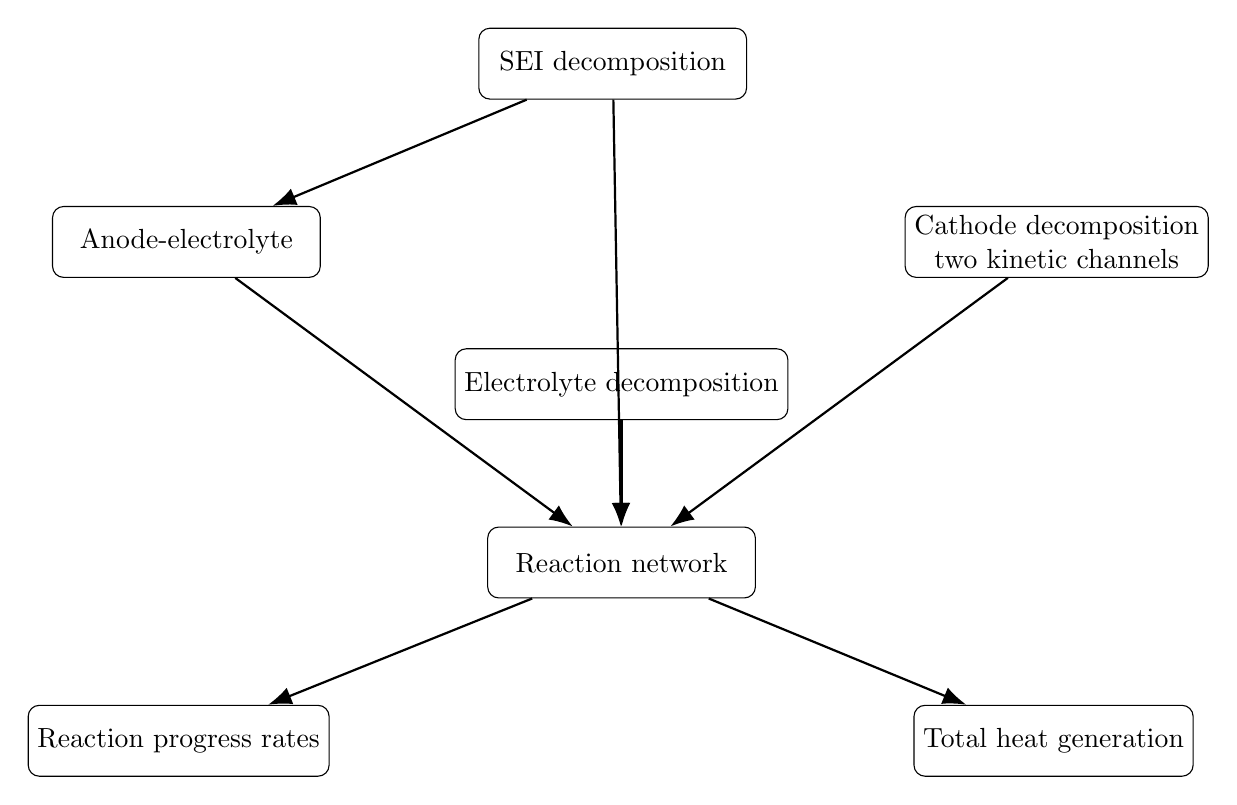
\begin{tikzpicture}[
        node distance=1.35cm and 2.0cm,
        block/.style={
            rectangle,
            rounded corners,
            draw,
            align=center,
            minimum width=3.4cm,
            minimum height=0.9cm
        },
        line/.style={
            -{Latex[length=3mm]},
            thick
        }
    ]

    \node[block] (sei) {SEI decomposition};

    \node[block, below left=of sei] (anode)
        {Anode-electrolyte};

    \node[block, below right=of sei] (cathode)
        {Cathode decomposition\\two kinetic channels};

    \node[block, below=of $(anode)!0.5!(cathode)$] (electrolyte)
        {Electrolyte decomposition};

    \node[block, below=of electrolyte] (network)
        {Reaction network};

    \node[block, below left=of network] (rates)
        {Reaction progress rates};

    \node[block, below right=of network] (heat)
        {Total heat generation};

    \draw[line] (sei) -- (anode);
    \draw[line] (sei) -- (network);
    \draw[line] (anode) -- (network);
    \draw[line] (cathode) -- (network);
    \draw[line] (electrolyte) -- (network);

    \draw[line] (network) -- (rates);
    \draw[line] (network) -- (heat);

    \end{tikzpicture}

    \caption{
        Representation of the Hu et al.\ thermal runaway model within
        the generic LiionTR reaction-network architecture.
    }
    \label{fig:hu_architecture}
\end{figure}

The arrow between the SEI and anode blocks indicates that the
anode-electrolyte reaction depends on the state of the SEI reaction.
The remaining reactions are assembled into the same network and coupled
through the common thermal state.


\subsection{Scope of the implementation}

The present implementation focuses on the reduced-order reaction and
heat-generation structure described by \textcite{hu2020inhibition}.

The LiionTR representation should therefore be distinguished from a
complete mechanistic electrochemical or thermochemical model.

In particular, the current Hu reaction network does not itself determine

\begin{itemize}
    \item equilibrium gas composition;
    \item gas-phase secondary reactions;
    \item electrochemical electrode potentials;
    \item spatial temperature distributions;
    \item mechanical deformation or rupture;
    \item multiphase vent products.
\end{itemize}

These phenomena are intended to be represented by separate LiionTR
subsystems or external scientific backends.

\section{Gas Generation}
\label{sec:gases}
Thermal runaway reactions can produce substantial quantities of gas.
LiionTR currently represents gas generation using a reduced-order
empirical formulation in which prescribed species yields are associated
with reaction progress.

This formulation provides the coupling required to study gas inventory,
internal pressure, and venting while keeping the gas-generation model
independent from the reaction kinetics and numerical solver.


\subsection{Gas species}

Each gas species $s$ is characterized by a molar mass

\begin{equation}
    M_s,
\end{equation}

expressed in \si{\kilogram\per\mole}.

The instantaneous gas state is represented by the mole inventory

\begin{equation}
    n_s,
\end{equation}

for each species.


\subsection{Gas inventory}

For a mixture containing $N_s$ species, the total gas amount is

\begin{equation}
    n_{\mathrm{tot}}
    =
    \sum_{s=1}^{N_s}
    n_s.
    \label{eq:gas_total_moles}
\end{equation}

The total gas mass is

\begin{equation}
    m_{\mathrm{gas}}
    =
    \sum_{s=1}^{N_s}
    n_s M_s.
    \label{eq:gas_total_mass}
\end{equation}

The mole fraction of species $s$ is

\begin{equation}
    x_s
    =
    \frac{
        n_s
    }{
        n_{\mathrm{tot}}
    },
    \label{eq:gas_mole_fraction}
\end{equation}

such that

\begin{equation}
    \sum_{s=1}^{N_s}
    x_s
    =
    1
\end{equation}

for a nonempty gas inventory.


\subsection{Mean molar mass}

The current venting model uses the mole-weighted mean molar mass

\begin{equation}
    \overline{M}
    =
    \sum_{s=1}^{N_s}
    x_s M_s.
    \label{eq:mean_molar_mass}
\end{equation}

Equivalently,

\begin{equation}
    \overline{M}
    =
    \frac{
        \displaystyle
        \sum_{s=1}^{N_s}
        n_s M_s
    }{
        \displaystyle
        \sum_{s=1}^{N_s}
        n_s
    }.
\end{equation}

This effective property provides the connection between the
species-resolved gas inventory and the single-mixture compressible-flow
model.


\subsection{Empirical reaction gas yields}

The current LiionTR gas-generation model assigns prescribed gas yields to
individual thermal runaway reactions.

For reaction $i$ and species $s$, the gas yield is denoted

\begin{equation}
    Y_{i,s},
\end{equation}

with units of

\begin{equation}
    \si{\mole\per\kilogram}
\end{equation}

of reacted material.

If reaction $i$ occupies an effective mass fraction $w_i$ of a cell with
mass $m_{\mathrm{cell}}$, the corresponding reacted-material rate is

\begin{equation}
    \frac{dm_{i,\mathrm{reacted}}}{dt}
    =
    m_{\mathrm{cell}}
    w_i
    \frac{d\alpha_i}{dt}.
    \label{eq:reacted_material_rate}
\end{equation}

The generation rate of species $s$ from reaction $i$ is therefore

\begin{equation}
    \dot{n}_{i,s}
    =
    Y_{i,s}
    m_{\mathrm{cell}}
    w_i
    \dot{\alpha}_i.
    \label{eq:species_generation_single_reaction}
\end{equation}


\subsection{Total species generation rate}

When multiple reactions generate the same gas species, their
contributions are summed.

The total generation rate of species $s$ is

\begin{equation}
    \dot{n}_{s,\mathrm{gen}}
    =
    \sum_{i=1}^{N_r}
    Y_{i,s}
    m_{\mathrm{cell}}
    w_i
    \dot{\alpha}_i,
    \label{eq:species_generation_total}
\end{equation}

where $N_r$ is the number of thermal runaway reactions.


\subsection{Cumulative gas generation}

If reaction $i$ evolves from an initial conversion
$\alpha_{i,0}$ to $\alpha_i$, the corresponding conversion change is

\begin{equation}
    \Delta \alpha_i
    =
    \alpha_i-\alpha_{i,0}.
\end{equation}

The cumulative gas amount associated with species $s$ is then

\begin{equation}
    n_{s,\mathrm{generated}}
    =
    \sum_{i=1}^{N_r}
    Y_{i,s}
    m_{\mathrm{cell}}
    w_i
    \left(
        \alpha_i-\alpha_{i,0}
    \right).
    \label{eq:cumulative_gas_generation}
\end{equation}

This expression is useful for closed-system calculations and for
verification of the integrated gas-generation rates.


\subsection{Closed-cell gas balance}

Before vent opening, all generated gas remains inside the modeled free
volume.

The species balance is

\begin{equation}
    \frac{dn_s}{dt}
    =
    \dot{n}_{s,\mathrm{gen}}.
    \label{eq:closed_gas_balance}
\end{equation}

The total mole inventory therefore increases according to

\begin{equation}
    \frac{dn_{\mathrm{tot}}}{dt}
    =
    \sum_s
    \dot{n}_{s,\mathrm{gen}}.
\end{equation}


\subsection{Gas balance after vent opening}

After vent opening, gas generation and gas discharge occur
simultaneously.

The species balance becomes

\begin{equation}
    \frac{dn_s}{dt}
    =
    \dot{n}_{s,\mathrm{gen}}
    -
    \dot{n}_{s,\mathrm{vent}}.
    \label{eq:open_gas_balance}
\end{equation}

The instantaneous gas composition may therefore evolve because of both
reaction-driven generation and removal through the vent.


\subsection{Coupling to pressure}

The gas inventory supplies the total gas amount used by the pressure
model.

For the current ideal-gas formulation,

\begin{equation}
    P
    =
    \frac{
        n_{\mathrm{tot}} R T
    }{
        V_{\mathrm{free}}
    }.
    \label{eq:gases_pressure_coupling}
\end{equation}

Thus, both gas generation and temperature evolution contribute directly
to cell pressurization.


\subsection{Coupling to venting}

The gas inventory also provides the mixture composition required by the
vent-flow model.

The mean molar mass is calculated using
\cref{eq:mean_molar_mass}, and the total molar discharge rate is
distributed between species according to their instantaneous mole
fractions.

This coupling is represented schematically in
\cref{fig:gas_architecture}.

\begin{figure}[htbp]
    \centering

    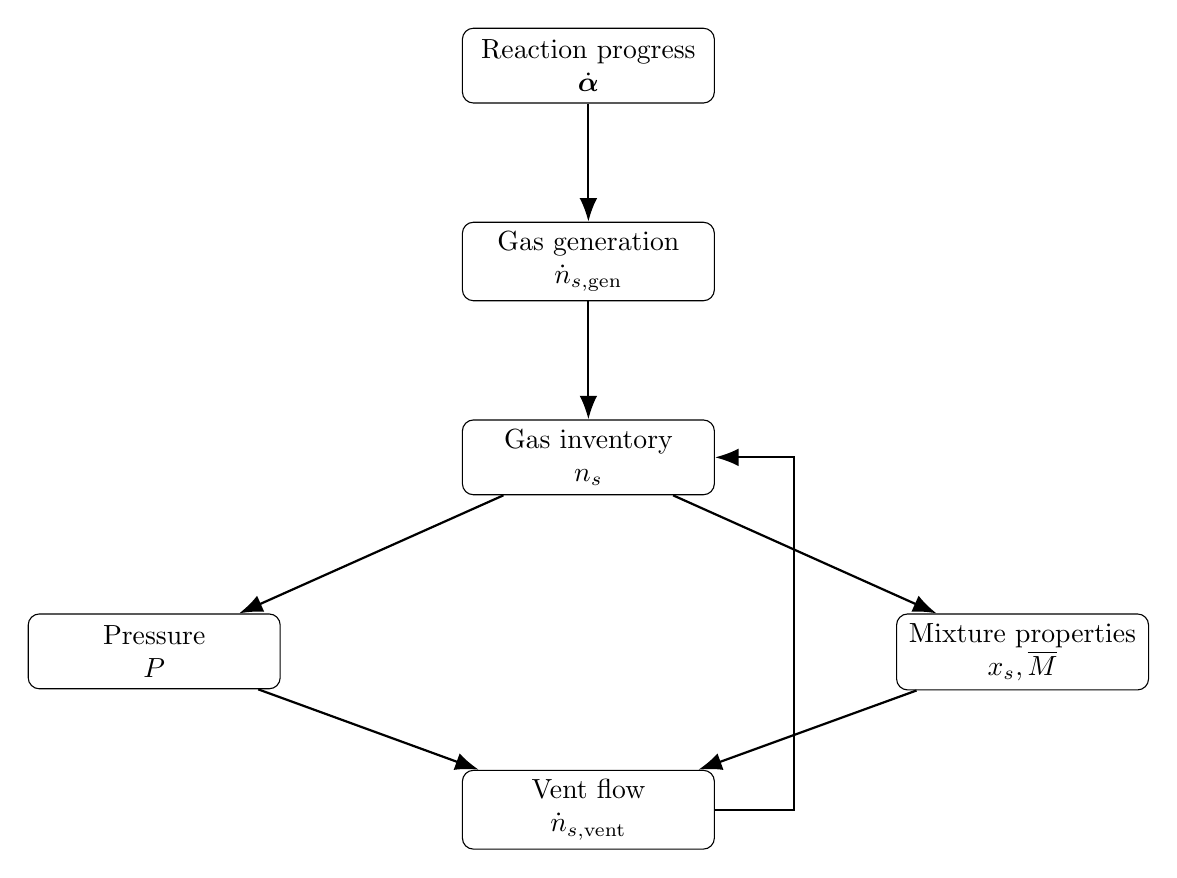
\begin{tikzpicture}[
        node distance=1.5cm and 2.3cm,
        block/.style={
            rectangle,
            rounded corners,
            draw,
            align=center,
            minimum width=3.2cm,
            minimum height=0.95cm
        },
        line/.style={
            -{Latex[length=3mm]},
            thick
        }
    ]

    \node[block] (reaction)
        {Reaction progress\\$\dot{\boldsymbol{\alpha}}$};

    \node[block, below=of reaction] (generation)
        {Gas generation\\$\dot{n}_{s,\mathrm{gen}}$};

    \node[block, below=of generation] (inventory)
        {Gas inventory\\$n_s$};

    \node[block, below left=of inventory] (pressure)
        {Pressure\\$P$};

    \node[block, below right=of inventory] (properties)
        {Mixture properties\\$x_s,\overline{M}$};

    \node[block, below=of $(pressure)!0.5!(properties)$] (vent)
        {Vent flow\\$\dot{n}_{s,\mathrm{vent}}$};

    \draw[line] (reaction) -- (generation);
    \draw[line] (generation) -- (inventory);
    \draw[line] (inventory) -- (pressure);
    \draw[line] (inventory) -- (properties);

    \draw[line] (pressure) -- (vent);
    \draw[line] (properties) -- (vent);

    \draw[line]
        (vent.east)
        -- ++(1.0,0)
        |- (inventory.east);

    \end{tikzpicture}

    \caption{
        Coupling between reaction-driven gas generation, the gas
        inventory, pressure, mixture properties, and vent discharge in
        the current LiionTR formulation.
    }
    \label{fig:gas_architecture}
\end{figure}


\subsection{Current assumptions}

The empirical gas-generation formulation assumes that:

\begin{itemize}
    \item gas yields are prescribed directly for individual reactions;
    \item species yields remain constant during each reaction;
    \item gas yields do not explicitly depend on temperature or pressure;
    \item gas-phase secondary chemistry is not represented;
    \item the gas mixture is spatially homogeneous;
    \item all gas species share a common temperature;
    \item the gas temperature is equal to the lumped cell temperature;
    \item condensation and phase separation are neglected;
    \item gas dissolution into condensed phases is neglected.
\end{itemize}


\subsection{Limitations of fixed species yields}

Thermal runaway gas composition can depend strongly on battery chemistry,
electrolyte composition, state of charge, temperature, pressure, and
secondary reactions.

Actual vent gases may contain, among other species,

\begin{equation}
    \mathrm{
        H_2,\,
        H_2O,\,
        CO,\,
        CO_2,\,
        CH_4,\,
        C_2H_4
    }.
\end{equation}

Additional fluorinated or phosphorus-containing species may also be
important depending on electrolyte chemistry.

A fixed species-yield model cannot generally predict these composition
changes from first principles.


\subsection{Future thermochemical formulation}

The intended long-term thermochemical architecture is to replace or
complement direct species yields with elemental source inventories.

Conceptually,

\begin{equation}
    \text{reaction progress}
    \longrightarrow
    \text{element inventory}
    \longrightarrow
    \text{chemical equilibrium}
    \longrightarrow
    \text{gas composition}.
\end{equation}

Relevant elemental inventories may include

\begin{equation}
    \mathrm{
        C,\,
        H,\,
        O,\,
        N,\,
        F,\,
        P,\,
        Li
    }.
\end{equation}

A thermochemical backend such as Cantera could then provide equilibrium
composition and mixture properties.

The present empirical implementation is retained because it provides a
simple, deterministic, and independently testable formulation while the
thermochemical architecture is developed.

\section{Pressure and Venting}
\label{sec:pressure-venting}
The gas-generation subsystem is coupled to internal pressure and venting
models in order to represent cell pressurization and subsequent gas
discharge.

The current formulation combines an ideal-gas pressure model with
compressible single-phase vent flow.


\subsection{Ideal-gas pressure}

The cell gas pressure is calculated using

\begin{equation}
    P
    V_{\mathrm{free}}
    =
    n_{\mathrm{tot}}
    R
    T,
\end{equation}

or

\begin{equation}
    P
    =
    \frac{
        n_{\mathrm{tot}}RT
    }{
        V_{\mathrm{free}}
    },
    \label{eq:pressure_ideal}
\end{equation}

where $V_{\mathrm{free}}$ is the available gas volume.

All pressures are treated as absolute pressures.


\subsection{Initial gas inventory}

The initial gas amount is calculated from the specified initial pressure
$P_0$, initial temperature $T_0$, and free volume:

\begin{equation}
    n_0
    =
    \frac{
        P_0 V_{\mathrm{free}}
    }{
        R T_0
    }.
    \label{eq:initial_gas_moles}
\end{equation}

Before venting, the total amount of gas can be represented as the sum of
the initial inventory and generated gas.

During venting, however, pressure must be reconstructed directly from the
instantaneous integrated species inventories.


\subsection{Pressure-temperature coupling}

For fixed volume,

\begin{equation}
    P
    \propto
    n_{\mathrm{tot}} T.
\end{equation}

Cell pressure can therefore rise because of both

\begin{enumerate}
    \item gas generation, which increases $n_{\mathrm{tot}}$;
    \item thermal runaway, which increases $T$.
\end{enumerate}

The pressure response is thus strongly coupled to the thermal and
reaction subsystems.


\subsection{Vent-opening criterion}

A vent-opening pressure

\begin{equation}
    P_{\mathrm{vent}}
\end{equation}

may be specified as part of the thermal problem.

The vent-opening event occurs when

\begin{equation}
    P
    =
    P_{\mathrm{vent}}.
    \label{eq:vent_open_condition}
\end{equation}

Before this condition is reached, the gas system is treated as closed.

After the event, the vent is considered permanently open.


\subsection{Maximum-pressure criterion}

An independent maximum-pressure threshold may also be specified,

\begin{equation}
    P_{\max}.
\end{equation}

This condition may be used to terminate numerical integration when

\begin{equation}
    P
    =
    P_{\max}.
    \label{eq:max_pressure_condition}
\end{equation}

The maximum-pressure threshold is distinct from the vent-opening
pressure and may represent a numerical safety criterion or a simplified
containment-failure limit.


\subsection{Compressible vent flow}

Gas discharge through the vent is represented using compressible
ideal-gas flow.

The upstream pressure is

\begin{equation}
    P_u
    =
    P_{\mathrm{cell}},
\end{equation}

while the downstream pressure is typically the ambient pressure,

\begin{equation}
    P_d
    =
    P_{\mathrm{ambient}}.
\end{equation}

The pressure ratio is

\begin{equation}
    r_p
    =
    \frac{
        P_d
    }{
        P_u
    }.
    \label{eq:pressure_ratio}
\end{equation}


\subsection{Specific gas constant}

The specific gas constant of the mixture is calculated as

\begin{equation}
    R_s
    =
    \frac{
        R
    }{
        \overline{M}
    },
    \label{eq:specific_gas_constant}
\end{equation}

where $\overline{M}$ is the instantaneous mean molar mass of the gas
mixture.


\subsection{Heat-capacity ratio}

The current vent model uses a prescribed heat-capacity ratio

\begin{equation}
    \gamma
    =
    \frac{
        c_p
    }{
        c_v
    }.
\end{equation}

In the present implementation, $\gamma$ is treated as constant rather
than being recomputed from the instantaneous gas composition.


\subsection{Critical pressure ratio}

For ideal-gas isentropic flow, the critical downstream-to-upstream
pressure ratio is

\begin{equation}
    r_{\mathrm{crit}}
    =
    \left(
        \frac{
            2
        }{
            \gamma+1
        }
    \right)^{
        \frac{
            \gamma
        }{
            \gamma-1
        }
    }.
    \label{eq:critical_pressure_ratio}
\end{equation}

The flow is considered choked when

\begin{equation}
    \frac{P_d}{P_u}
    \leq
    r_{\mathrm{crit}}.
    \label{eq:choked_condition}
\end{equation}


\subsection{Choked mass flow}

For choked flow, the mass discharge rate is

\begin{equation}
    \dot{m}_{\mathrm{vent}}
    =
    C_d A_v P_u
    \sqrt{
        \frac{\gamma}{R_s T}
    }
    \left(
        \frac{2}{\gamma+1}
    \right)^{
        \frac{\gamma+1}{2(\gamma-1)}
    }.
    \label{eq:choked_mass_flow}
\end{equation}

where $C_d$ is the discharge coefficient and $A_v$ is the effective vent
area.

Once the flow is choked, decreasing downstream pressure further does not
increase the mass flow predicted by this relation.


\subsection{Unchoked mass flow}

When

\begin{equation}
    \frac{P_d}{P_u}
    >
    r_{\mathrm{crit}},
\end{equation}

the discharge is treated as unchoked.

The mass flow rate is

\begin{equation}
    \dot{m}_{\mathrm{vent}}
    =
    C_d A_v P_u
    \sqrt{
        \frac{2\gamma}
             {R_s T(\gamma-1)}
        \left[
            \left(
                \frac{P_d}{P_u}
            \right)^{2/\gamma}
            -
            \left(
                \frac{P_d}{P_u}
            \right)^{(\gamma+1)/\gamma}
        \right]
    }.
    \label{eq:unchoked_mass_flow}
\end{equation}

As $P_d$ approaches $P_u$, the predicted discharge rate approaches zero.


\subsection{Reverse flow}

The current formulation does not represent inward flow through the vent.

Consequently,

\begin{equation}
    P_u
    \leq
    P_d
    \quad
    \Longrightarrow
    \quad
    \dot{m}_{\mathrm{vent}}
    =
    0.
    \label{eq:no_reverse_flow}
\end{equation}


\subsection{Molar vent flow}

The total mass discharge rate is converted to a molar flow rate using

\begin{equation}
    \dot{n}_{\mathrm{vent}}
    =
    \frac{
        \dot{m}_{\mathrm{vent}}
    }{
        \overline{M}
    }.
    \label{eq:total_molar_vent_flow}
\end{equation}


\subsection{Species vent rates}

The current model assumes a well-mixed gas inventory.

The vented gas therefore has the same mole fractions as the gas
remaining inside the modeled free volume.

For species $s$,

\begin{equation}
    \dot{n}_{s,\mathrm{vent}}
    =
    x_s
    \dot{n}_{\mathrm{vent}}.
    \label{eq:species_vent_flow}
\end{equation}

Summing over species gives

\begin{equation}
    \sum_s
    \dot{n}_{s,\mathrm{vent}}
    =
    \dot{n}_{\mathrm{vent}}.
\end{equation}


\subsection{Closed and open governing equations}

The vent model creates two distinct gas-balance phases.

Before vent opening,

\begin{equation}
    \frac{dn_s}{dt}
    =
    \dot{n}_{s,\mathrm{gen}}.
    \label{eq:vent_closed_phase}
\end{equation}

After vent opening,

\begin{equation}
    \frac{dn_s}{dt}
    =
    \dot{n}_{s,\mathrm{gen}}
    -
    \dot{n}_{s,\mathrm{vent}}.
    \label{eq:vent_open_phase}
\end{equation}


\subsection{Irreversible vent transition}

The current LiionTR implementation treats vent opening as an irreversible
state transition,

\begin{equation}
    \mathrm{CLOSED}
    \longrightarrow
    \mathrm{OPEN}.
\end{equation}

The vent does not reseal if pressure subsequently falls below
$P_{\mathrm{vent}}$.

The numerical interpretation of this transition is illustrated in
\cref{fig:vent_state_machine}.

\begin{figure}[htbp]
    \centering

    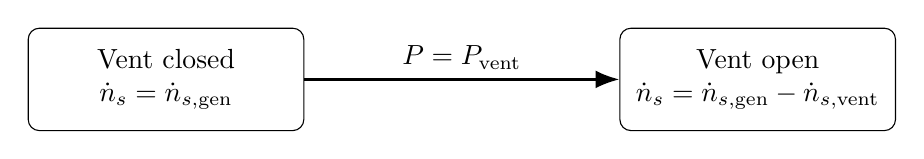
\begin{tikzpicture}[
        node distance=4.0cm,
        state/.style={
            rectangle,
            rounded corners,
            draw,
            align=center,
            minimum width=3.5cm,
            minimum height=1.3cm
        },
        line/.style={
            -{Latex[length=3mm]},
            thick
        }
    ]

    \node[state] (closed)
        {Vent closed\\
         $\dot{n}_s=\dot{n}_{s,\mathrm{gen}}$};

    \node[state, right=of closed] (open)
        {Vent open\\
         $\dot{n}_s=
         \dot{n}_{s,\mathrm{gen}}
         -
         \dot{n}_{s,\mathrm{vent}}$};

    \draw[line]
        (closed)
        --
        node[above, align=center]
        {$P=P_{\mathrm{vent}}$}
        (open);

    \end{tikzpicture}

    \caption{
        Irreversible vent-state transition used by the current LiionTR
        solver.
    }
    \label{fig:vent_state_machine}
\end{figure}


\subsection{Coupled pressure-vent feedback}

After vent opening, pressure determines the vent-flow rate, while the
vent-flow rate modifies the gas inventory and therefore pressure.

This feedback may be represented as

\begin{equation}
    P
    \longrightarrow
    \dot{n}_{\mathrm{vent}}
    \longrightarrow
    n_{\mathrm{tot}}
    \longrightarrow
    P.
\end{equation}

Gas generation and temperature continue to evolve simultaneously.

The pressure response therefore depends on the competition between

\begin{equation}
    \dot{n}_{\mathrm{gen}}
\end{equation}

and

\begin{equation}
    \dot{n}_{\mathrm{vent}},
\end{equation}

together with the evolving thermal state.


\subsection{Current assumptions}

The pressure and venting formulation assumes:

\begin{itemize}
    \item ideal-gas behavior;
    \item constant free volume;
    \item uniform gas pressure;
    \item gas temperature equal to the lumped cell temperature;
    \item single-phase gas discharge;
    \item quasi-steady compressible vent flow;
    \item fixed effective vent area;
    \item constant discharge coefficient;
    \item constant heat-capacity ratio;
    \item a well-mixed gas inventory;
    \item no preferential species transport through the vent;
    \item no reverse flow;
    \item irreversible vent opening.
\end{itemize}


\subsection{Limitations}

Real lithium-ion battery venting can involve considerably more complex
behavior than represented by the present model.

The discharged material may contain

\begin{itemize}
    \item permanent gases;
    \item electrolyte vapor;
    \item liquid droplets;
    \item aerosols;
    \item condensed particles;
    \item decomposed electrode and separator material.
\end{itemize}

The physical vent may also deform progressively, resulting in a
time-dependent effective flow area.

These mechanisms are outside the scope of the present reduced-order
model.


\subsection{Future extensions}

Future developments may include:

\begin{itemize}
    \item gas properties obtained dynamically from Cantera;
    \item temperature- and composition-dependent $\gamma$;
    \item variable vent geometry;
    \item progressive vent opening;
    \item mechanical rupture models;
    \item two-phase and multiphase discharge;
    \item electrolyte flashing;
    \item vent-jet momentum models;
    \item combustion and fire models downstream of the vent.
\end{itemize}

\section{Numerical Method}
\label{sec:numerical-method}
LiionTR formulates thermal runaway as a coupled system of ordinary
differential equations integrated in time.

The numerical solver owns the complete dynamic state and evaluates the
physical models only as functions of the current state. This avoids
hidden mutable state inside the thermal, reaction, gas, pressure, and
venting models.


\subsection{State vector}

For a problem containing $N_r$ reaction states and $N_s$ gas species,
the integrated state vector is

\begin{equation}
    \mathbf{y}
    =
    \begin{bmatrix}
        T &
        \alpha_1 &
        \cdots &
        \alpha_{N_r} &
        n_1 &
        \cdots &
        n_{N_s}
    \end{bmatrix}^{\mathrm{T}}.
    \label{eq:numerical_state_vector}
\end{equation}

The first component is the lumped cell temperature.

The following $N_r$ components contain reaction conversions,

\begin{equation}
    \boldsymbol{\alpha}
    =
    \begin{bmatrix}
        \alpha_1 &
        \cdots &
        \alpha_{N_r}
    \end{bmatrix}^{\mathrm{T}},
\end{equation}

while the final $N_s$ components contain the gas-species inventories,

\begin{equation}
    \mathbf{n}
    =
    \begin{bmatrix}
        n_1 &
        \cdots &
        n_{N_s}
    \end{bmatrix}^{\mathrm{T}}.
\end{equation}

When gas generation is disabled, the gas portion of the state vector is
absent.


\subsection{Initial conditions}

The initial numerical state is assembled from the configured thermal
problem.

The temperature is initialized as

\begin{equation}
    T(0)
    =
    T_0.
\end{equation}

Each reaction is initialized according to its prescribed initial
conversion,

\begin{equation}
    \alpha_i(0)
    =
    \alpha_{i,0}.
\end{equation}

When gas modeling is enabled, the initial gas inventory is determined
from the configured species inventory or from the pressure model.

The complete initial state is therefore

\begin{equation}
    \mathbf{y}(0)
    =
    \mathbf{y}_0.
\end{equation}


\subsection{Right-hand-side evaluation}

At every solver evaluation, the current state vector is unpacked into
temperature, reaction conversions, and gas inventories.

The reaction context is constructed from the current conversion vector,

\begin{equation}
    \boldsymbol{\alpha}(t).
\end{equation}

The reaction network then evaluates

\begin{equation}
    \dot{\boldsymbol{\alpha}}
    =
    \mathbf{f}_{\alpha}
    \left(
        T,
        \boldsymbol{\alpha}
    \right).
    \label{eq:rhs_reaction_rates}
\end{equation}

The corresponding total reaction heat is

\begin{equation}
    \dot{Q}_{\mathrm{gen}}
    =
    \dot{Q}_{\mathrm{gen}}
    \left(
        T,
        \boldsymbol{\alpha}
    \right).
\end{equation}

The thermal model evaluates

\begin{equation}
    \dot{T}
    =
    \frac{
        \dot{Q}_{\mathrm{gen}}
        -
        hA(T-T_{\infty})
    }{
        C_{\mathrm{th}}
    }.
    \label{eq:rhs_temperature}
\end{equation}


\subsection{Gas-generation contribution}

If a gas-generation model is present, the reaction rates are also used
to determine species-generation rates,

\begin{equation}
    \dot{\mathbf{n}}_{\mathrm{gen}}
    =
    \mathbf{f}_{\mathrm{gas}}
    \left(
        \dot{\boldsymbol{\alpha}}
    \right).
    \label{eq:rhs_gas_generation}
\end{equation}

Before vent opening,

\begin{equation}
    \dot{\mathbf{n}}
    =
    \dot{\mathbf{n}}_{\mathrm{gen}}.
    \label{eq:rhs_closed_gas}
\end{equation}


\subsection{Pressure reconstruction}

Internal pressure is not integrated as an independent state variable.

Instead, it is reconstructed algebraically from the instantaneous gas
inventory and temperature,

\begin{equation}
    P
    =
    P
    \left(
        T,
        \mathbf{n}
    \right).
    \label{eq:pressure_algebraic_state}
\end{equation}

For the current ideal-gas formulation,

\begin{equation}
    P
    =
    \frac{
        R T
        \displaystyle\sum_s n_s
    }{
        V_{\mathrm{free}}
    }.
\end{equation}

Avoiding pressure as an additional integrated variable ensures direct
consistency between pressure and gas inventory.


\subsection{Vent-opening event}

When venting is enabled, the closed-cell integration defines an event
function

\begin{equation}
    g_{\mathrm{vent}}
    \left(
        t,
        \mathbf{y}
    \right)
    =
    P
    \left(
        T,
        \mathbf{n}
    \right)
    -
    P_{\mathrm{vent}}.
    \label{eq:vent_event_function}
\end{equation}

Vent opening occurs when

\begin{equation}
    g_{\mathrm{vent}}
    =
    0.
\end{equation}

The event terminates the closed-cell integration.


\subsection{Two-phase integration}

The current solver represents irreversible vent opening using two
successive numerical integrations.

The first phase solves the closed-cell system,

\begin{equation}
    \dot{\mathbf{y}}
    =
    \mathbf{F}_{\mathrm{closed}}
    \left(
        t,
        \mathbf{y}
    \right),
\end{equation}

until either the final time or a terminating event is reached.

If the vent-opening event occurs, the state at the event time

\begin{equation}
    \mathbf{y}_{\mathrm{vent}}
\end{equation}

becomes the initial condition of the second phase.

The second integration solves

\begin{equation}
    \dot{\mathbf{y}}
    =
    \mathbf{F}_{\mathrm{open}}
    \left(
        t,
        \mathbf{y}
    \right),
\end{equation}

where the gas balance is modified to include vent discharge,

\begin{equation}
    \dot{\mathbf{n}}
    =
    \dot{\mathbf{n}}_{\mathrm{gen}}
    -
    \dot{\mathbf{n}}_{\mathrm{vent}}.
    \label{eq:rhs_open_gas}
\end{equation}


\subsection{Solver flow}

The numerical sequence is summarized in
\cref{fig:solver_flow}.

\begin{figure}[htbp]
    \centering

    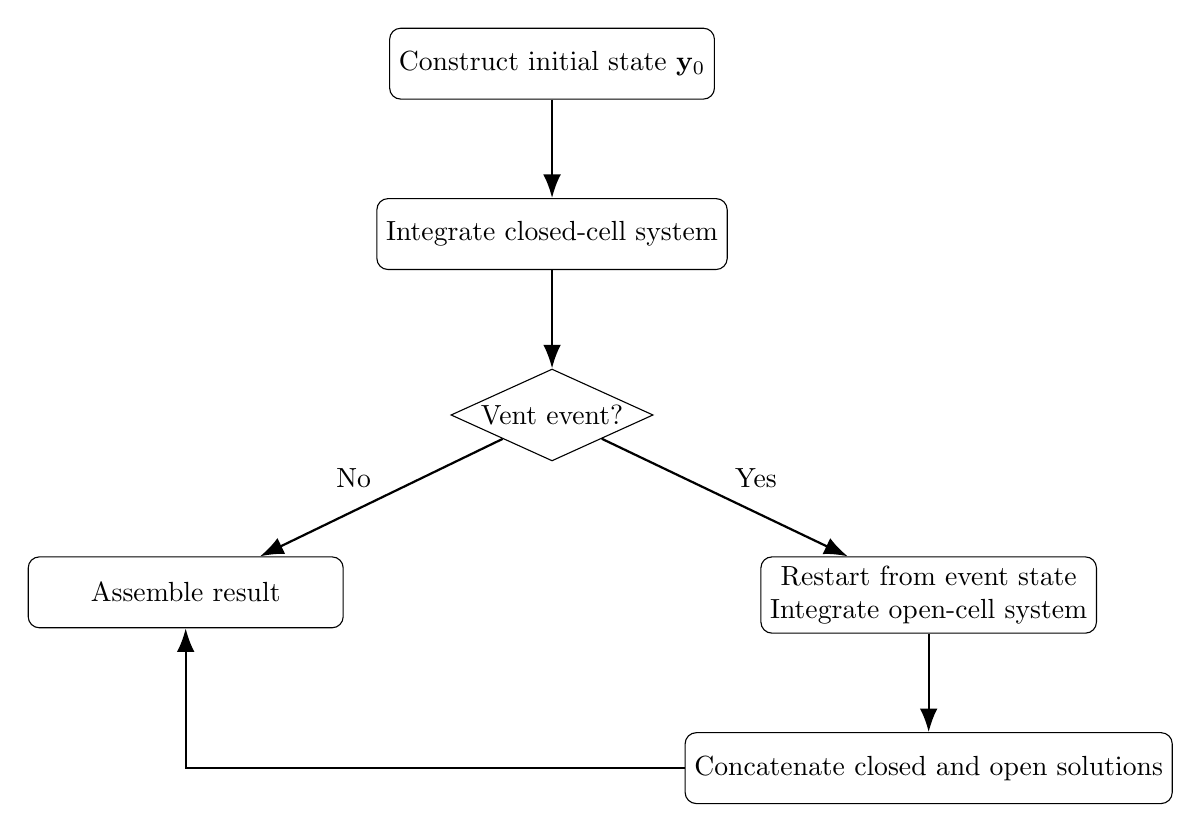
\begin{tikzpicture}[
        node distance=1.25cm and 2.0cm,
        block/.style={
            rectangle,
            rounded corners,
            draw,
            align=center,
            minimum width=4.0cm,
            minimum height=0.9cm
        },
        decision/.style={
            diamond,
            draw,
            align=center,
            aspect=2.2,
            inner sep=1pt
        },
        line/.style={
            -{Latex[length=3mm]},
            thick
        }
    ]

    \node[block] (initial)
        {Construct initial state $\mathbf{y}_0$};

    \node[block, below=of initial] (closed)
        {Integrate closed-cell system};

    \node[decision, below=of closed] (ventevent)
        {Vent event?};

    \node[block, below left=1.5cm and 2.0cm of ventevent] (finish)
        {Assemble result};

    \node[block, below right=1.5cm and 2.0cm of ventevent] (open)
        {Restart from event state\\
         Integrate open-cell system};

    \node[block, below=of open] (merge)
        {Concatenate closed and open solutions};

    \draw[line] (initial) -- (closed);
    \draw[line] (closed) -- (ventevent);

    \draw[line]
        (ventevent)
        --
        node[above left] {No}
        (finish);

    \draw[line]
        (ventevent)
        --
        node[above right] {Yes}
        (open);

    \draw[line] (open) -- (merge);
    \draw[line] (merge.west) -| (finish.south);

    \end{tikzpicture}

    \caption{
        Numerical integration strategy used for irreversible vent
        opening in the current LiionTR solver.
    }
    \label{fig:solver_flow}
\end{figure}


\subsection{Maximum-temperature event}

A maximum permitted temperature may be specified as

\begin{equation}
    T_{\max}.
\end{equation}

The corresponding event function is

\begin{equation}
    g_T
    =
    T-T_{\max}.
    \label{eq:max_temperature_event}
\end{equation}

The integration terminates when the event crosses zero in the prescribed
direction.


\subsection{Maximum-pressure event}

Similarly, a maximum-pressure event is represented by

\begin{equation}
    g_P
    =
    P-P_{\max}.
    \label{eq:max_pressure_event}
\end{equation}

This event can terminate either the closed or open phase of the
simulation.


\subsection{Stiff numerical integration}

Thermal runaway kinetics frequently contain strongly temperature-sensitive
Arrhenius terms spanning several orders of magnitude.

The coupled equations can consequently become stiff, particularly during
the rapid acceleration preceding thermal runaway.

The default LiionTR solver therefore uses the backward differentiation
formula method available through SciPy's \texttt{solve\_ivp} interface
\parencite{virtanen2020scipy}.

The BDF method is an implicit variable-order integration method suitable
for stiff ordinary differential equations.


\subsection{Adaptive time stepping}

The solver automatically adjusts its internal time step according to
local error estimates.

The user may specify relative and absolute tolerances,

\begin{equation}
    \mathrm{rtol}
\end{equation}

and

\begin{equation}
    \mathrm{atol},
\end{equation}

as well as an optional maximum time step.

The internal time-step size can become substantially smaller during the
rapid thermal runaway phase than during the initial slow-heating period.


\subsection{State reconstruction}

After numerical integration, the resulting solver state is separated
into physically meaningful output quantities.

These include

\begin{itemize}
    \item time;
    \item cell temperature;
    \item individual reaction conversions;
    \item reaction progress rates;
    \item heat-generation rates;
    \item gas-species inventories;
    \item total gas amount;
    \item gas composition;
    \item pressure;
    \item vent status.
\end{itemize}

For vented simulations, the two numerical phases are concatenated into a
single continuous simulation result.


\subsection{Numerical architecture}

The numerical solver acts as the orchestration layer between the
individual physical models.

Conceptually,

\begin{equation}
    \mathbf{y}
    \longrightarrow
    \begin{cases}
        \text{reaction model},\\
        \text{thermal model},\\
        \text{gas model},\\
        \text{pressure model},\\
        \text{vent model}
    \end{cases}
    \longrightarrow
    \dot{\mathbf{y}}.
\end{equation}

Individual physical components therefore remain independent of the
specific numerical integration algorithm.


\subsection{Current limitations}

The current numerical formulation assumes:

\begin{itemize}
    \item a single lumped temperature state;
    \item scalar reaction conversions;
    \item species-resolved gas inventories;
    \item pressure reconstructed algebraically;
    \item instantaneous transition from closed to fully open vent;
    \item no resealing after vent opening;
    \item no differential-algebraic constraints beyond algebraic
          reconstruction of derived quantities;
    \item no spatial discretization.
\end{itemize}


\subsection{Future numerical extensions}

Future developments may include:

\begin{itemize}
    \item alternative stiff and non-stiff integrators;
    \item explicit Jacobian evaluation;
    \item sparse Jacobian support;
    \item differential-algebraic formulations;
    \item adaptive vent-opening models;
    \item integration of internal energy instead of temperature;
    \item spatial thermal discretization;
    \item cell-to-cell propagation systems;
    \item sensitivity equations and parameter estimation.
\end{itemize}

\section{Verification}
\label{sec:verification}
Verification of LiionTR focuses on determining whether the implemented
numerical models reproduce their intended mathematical formulations.

This distinction is important:

\begin{itemize}
    \item \emph{verification} evaluates whether the equations are solved
          and implemented correctly;
    \item \emph{validation} evaluates whether those equations reproduce
          physical experimental behavior.
\end{itemize}

The current development stage places primary emphasis on verification.


\subsection{Unit-level verification}

Individual LiionTR components are tested independently wherever
possible.

The test suite includes checks for:

\begin{itemize}
    \item geometric quantities;
    \item material properties;
    \item cell mass and thermal capacity;
    \item kinetic-rate calculations;
    \item reaction-progress laws;
    \item reaction heat generation;
    \item reaction-network aggregation;
    \item gas inventory properties;
    \item gas-generation rates;
    \item ideal-gas pressure;
    \item choked and unchoked vent flow;
    \item event handling;
    \item coupled numerical simulations.
\end{itemize}

Unit-level testing is particularly important because the modular
architecture permits most physical components to be evaluated without
running a complete thermal runaway simulation.


\subsection{Dimensional consistency}

All internal physical quantities are represented in SI units.

Typical units include

\begin{align}
    T &: \si{\kelvin},
    \\
    P &: \si{\pascal},
    \\
    E_a &: \si{\joule\per\mole},
    \\
    \Delta H &: \si{\joule\per\kilogram},
    \\
    W &: \si{\kilogram\per\meter\cubed},
    \\
    \dot{Q} &: \si{\watt},
    \\
    n &: \si{\mole}.
\end{align}

Literature parameters reported in alternative units are explicitly
converted before construction of the corresponding LiionTR models.


\subsection{Reaction-energy consistency}

For a reaction with effective mass fraction $w$, reaction enthalpy
$\Delta H$, and conversion change

\begin{equation}
    \Delta \alpha
    =
    \alpha_f-\alpha_0,
\end{equation}

the expected specific energy release relative to total cell mass is

\begin{equation}
    q_{\mathrm{expected}}
    =
    w
    \Delta H
    \Delta\alpha.
    \label{eq:verification_expected_energy}
\end{equation}

For a complete reaction network,

\begin{equation}
    q_{\mathrm{expected,total}}
    =
    \sum_i
    w_i
    \Delta H_i
    \Delta\alpha_i,
    \label{eq:verification_total_energy}
\end{equation}

with the appropriate extension for multi-channel reactions.

Numerically integrating the heat-generation rate provides

\begin{equation}
    q_{\mathrm{integrated}}
    =
    \frac{1}{m_{\mathrm{cell}}}
    \int
    \dot{Q}_{\mathrm{gen}}
    \,dt.
    \label{eq:verification_integrated_energy}
\end{equation}

Agreement between
\cref{eq:verification_total_energy,eq:verification_integrated_energy}
provides an important consistency check between reaction progress and
heat generation.

\subsection{Thermal energy-balance closure}

A global energy-balance check was performed for the Hu et al.\
reference simulation.

For the lumped thermal formulation, integration over the simulation
interval gives

\begin{equation}
    q_{\mathrm{reaction}}
    =
    \Delta u_{\mathrm{sensible}}
    +
    q_{\mathrm{conv}}
    +
    \varepsilon_E,
\end{equation}

where $\varepsilon_E$ represents the numerical energy-balance residual.

The resulting balance is given in
\cref{tab:hu_energy_balance}.

\input{generated/hu2020_energy_balance}



A small residual demonstrates consistency between the integrated
reaction heat generation, the temperature evolution, and the
convective heat transfer computed by the lumped thermal model.

Because the reaction and convective energies are reconstructed by
numerical quadrature from the adaptive solver output, the residual
reflects both integration error and post-processing quadrature error.
It should therefore be interpreted as a numerical consistency metric
rather than as an independent physical validation.

The cumulative energy balance is shown in
\cref{fig:hu_cumulative_energy_balance}.

\begin{figure}[htbp]
    \centering
    \includegraphics[
        width=0.82\textwidth
    ]{hu2020_energy_balance_cumulative.pdf}

    \caption{
        Cumulative energy-balance closure for the Hu et al.\
        reference simulation. The cumulative reaction energy is
        compared with the sum of the sensible-energy increase and
        convective heat loss.
    }
    \label{fig:hu_cumulative_energy_balance}
\end{figure}

The near-superposition of the cumulative reaction energy and the
accounted thermal energy provides a direct visual verification of the
implemented lumped thermal balance.

\subsection{Hu model energy check}

A representative numerical simulation of the implemented Hu et al.\
reaction network was performed from an elevated initial temperature in
order to activate the thermal runaway mechanism.

For the tested case, the integrated specific reaction energy was

\begin{equation}
    q_{\mathrm{integrated}}
    \approx
    \SI{386.6}{\kilo\joule\per\kilogram}.
\end{equation}

The integrated heat release was consistent with the energy obtained from
the change in reaction states and the corresponding reaction
enthalpies.

This test verifies the internal consistency of the implemented reaction
network and heat-generation calculation. It should not be interpreted as
experimental validation of the Hu model.


\subsection{Thermal-response consistency}

For an adiabatic system with constant heat capacity and no heat loss,

\begin{equation}
    C_{\mathrm{th}}
    \frac{dT}{dt}
    =
    \dot{Q}_{\mathrm{gen}}.
\end{equation}

Integrating gives

\begin{equation}
    \Delta T
    =
    \frac{
        Q_{\mathrm{gen}}
    }{
        C_{\mathrm{th}}
    }.
    \label{eq:verification_adiabatic_temperature}
\end{equation}

This relationship provides a direct verification target for simplified
thermal problems.


\subsection{Gas-generation conservation}

For a closed system with no venting, the numerically integrated gas
inventory should agree with the cumulative reaction-yield relation.

For species $s$,

\begin{equation}
    n_s(t)
    -
    n_s(0)
    =
    \sum_i
    Y_{i,s}
    m_{\mathrm{cell}}
    w_i
    \left[
        \alpha_i(t)-\alpha_i(0)
    \right].
    \label{eq:verification_gas_conservation}
\end{equation}

Agreement verifies consistency between reaction progress, gas-generation
rates, and integrated species inventories.


\subsection{Pressure verification}

For a closed ideal-gas problem, pressure reconstructed from the numerical
state must satisfy

\begin{equation}
    P
    =
    \frac{
        n_{\mathrm{tot}}RT
    }{
        V_{\mathrm{free}}
    }.
\end{equation}

Synthetic problems with constant temperature or constant gas amount can
therefore be compared directly against analytical pressure evolution.


\subsection{Vent-flow verification}

The venting implementation is tested separately in both compressible-flow
regimes.

For

\begin{equation}
    \frac{P_d}{P_u}
    \leq
    r_{\mathrm{crit}},
\end{equation}

the choked-flow expression must be selected.

For

\begin{equation}
    \frac{P_d}{P_u}
    >
    r_{\mathrm{crit}},
\end{equation}

the unchoked-flow expression must be selected.

The model also verifies that

\begin{equation}
    P_u
    \leq
    P_d
\end{equation}

produces zero outward discharge.


\subsection{Vented coupled simulation}

A synthetic coupled simulation has been used to verify the complete
sequence

\begin{equation}
    \text{reaction}
    \rightarrow
    \text{heat}
    \rightarrow
    T
    \rightarrow
    \text{gas generation}
    \rightarrow
    P
    \rightarrow
    \text{vent opening}
    \rightarrow
    \text{gas discharge}.
\end{equation}

The test demonstrates that:

\begin{enumerate}
    \item reaction progress generates heat;
    \item heat generation increases temperature;
    \item reaction progress generates gas;
    \item gas accumulation and heating increase pressure;
    \item the vent opens when the prescribed pressure is reached;
    \item the solver transitions irreversibly to the open-vent system;
    \item gas discharge reduces the internal inventory;
    \item pressure approaches the downstream pressure after the dominant
          gas-generation period.
\end{enumerate}

This synthetic problem is designed to verify model coupling and event
handling rather than reproduce a particular commercial battery cell.


\subsection{Regression testing}

Automated regression tests are used to detect unintended changes in
physical behavior as the codebase evolves.

This is particularly important for coupled models because a local
software modification can alter:

\begin{itemize}
    \item reaction rates;
    \item integrated reaction energy;
    \item event times;
    \item maximum temperature;
    \item pressure evolution;
    \item vent discharge.
\end{itemize}

Regression tests therefore complement analytical unit tests.


\subsection{Verification hierarchy}

The current verification strategy follows the hierarchy illustrated in
\cref{fig:verification_hierarchy}.

\begin{figure}[htbp]
    \centering

    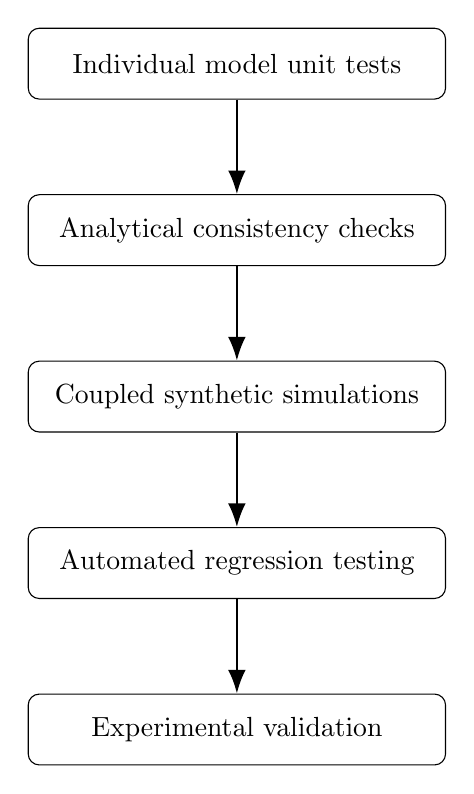
\begin{tikzpicture}[
        node distance=1.2cm,
        block/.style={
            rectangle,
            rounded corners,
            draw,
            align=center,
            minimum width=5.3cm,
            minimum height=0.9cm
        },
        line/.style={
            -{Latex[length=3mm]},
            thick
        }
    ]

    \node[block] (units)
        {Individual model unit tests};

    \node[block, below=of units] (analytic)
        {Analytical consistency checks};

    \node[block, below=of analytic] (coupled)
        {Coupled synthetic simulations};

    \node[block, below=of coupled] (regression)
        {Automated regression testing};

    \node[block, below=of regression] (validation)
        {Experimental validation};

    \draw[line] (units) -- (analytic);
    \draw[line] (analytic) -- (coupled);
    \draw[line] (coupled) -- (regression);
    \draw[line] (regression) -- (validation);

    \end{tikzpicture}

    \caption{
        Verification and validation hierarchy intended for LiionTR.
        Experimental validation represents a future development stage
        following verification of the numerical implementation.
    }
    \label{fig:verification_hierarchy}
\end{figure}


\subsection{Experimental validation}

Experimental validation remains an essential future step.

Relevant validation data may include:

\begin{itemize}
    \item differential scanning calorimetry measurements;
    \item accelerating rate calorimetry measurements;
    \item cell-surface temperature histories;
    \item pressure measurements;
    \item vent-opening times;
    \item total vented gas quantities;
    \item gas-composition measurements;
    \item abuse-test thermal runaway onset temperatures.
\end{itemize}

The modular structure of LiionTR is intended to allow kinetic,
thermochemical, pressure, and venting submodels to be calibrated and
validated independently before complete-cell validation is attempted.

\subsection{Coupled gas-pressure-venting verification}

The coupled gas-generation, pressure, and venting implementation was
evaluated using a deliberately simplified synthetic problem.

The purpose of this calculation is not to represent a physically
realistic lithium-ion cell, but to exercise the complete numerical
coupling

\begin{equation}
    \text{reaction}
    \rightarrow
    \text{gas generation}
    \rightarrow
    \text{pressure increase}
    \rightarrow
    \text{vent opening}
    \rightarrow
    \text{depressurization}.
\end{equation}

The model contains a single synthetic exothermic reaction producing
\ce{CO2}. The initial gas inventory consists primarily of \ce{N2} at
atmospheric pressure. The free gas volume is
\SI{1.0e-6}{\meter\cubed}, and the vent-opening pressure is prescribed as

\begin{equation}
    P_{\mathrm{vent}}
    =
    \SI{200}{\kilo\pascal}.
\end{equation}

The vent model uses an effective opening area of
\SI{1.0e-5}{\meter\squared}, a discharge coefficient of 0.8, and a
heat-capacity ratio of 1.30.

\input{generated/synthetic_vent_results}

The simulated vent opens at

\begin{equation}
    t_{\mathrm{vent}}
    =
    \SI{\SyntheticVentOpenTime}{\second},
\end{equation}

when the internal pressure reaches approximately

\begin{equation}
    P_{\max}
    =
    \SI{\SyntheticVentPeakPressure}{\kilo\pascal}.
\end{equation}

The pressure evolution is shown in
\cref{fig:synthetic_vent_pressure}.

\begin{figure}[htbp]
    \centering
    \includegraphics[
        width=0.82\textwidth
    ]{synthetic_vent_pressure.pdf}

    \caption{
        Internal pressure during the synthetic venting verification
        problem. The vent opens when the prescribed pressure threshold
        is reached, after which the internal pressure rapidly approaches
        the downstream ambient pressure.
    }
    \label{fig:synthetic_vent_pressure}
\end{figure}

At the end of the simulation, the vented system reaches

\begin{equation}
    P_f
    =
    \SI{\SyntheticVentFinalPressure}{\kilo\pascal},
\end{equation}

which is close to the prescribed downstream pressure of
\SI{101.325}{\kilo\pascal}.

For comparison, suppressing the vent while leaving the remaining model
unchanged produces a final pressure of

\begin{equation}
    P_{f,\mathrm{closed}}
    =
    \SI{\SyntheticClosedFinalPressure}{\kilo\pascal}.
\end{equation}

The very large closed-system pressure is a consequence of the
intentionally aggressive synthetic gas-generation rate and small free
volume. It should not be interpreted as a prediction for a physical
lithium-ion cell.

The internal gas inventory is shown in
\cref{fig:synthetic_vent_inventory}.

\begin{figure}[htbp]
    \centering
    \includegraphics[
        width=0.82\textwidth
    ]{synthetic_vent_gas_inventory.pdf}

    \caption{
        Internal \ce{N2}, \ce{CO2}, and total gas inventories during
        the synthetic venting verification problem.
    }
    \label{fig:synthetic_vent_inventory}
\end{figure}

Following vent opening, the internal gas inventory decreases as gas is
discharged through the vent. The corresponding reconstructed mass-flow
rate is shown in
\cref{fig:synthetic_vent_flow}.

\begin{figure}[htbp]
    \centering
    \includegraphics[
        width=0.82\textwidth
    ]{synthetic_vent_flow.pdf}

    \caption{
        Reconstructed vent mass-flow rate during the synthetic
        gas-pressure-venting verification problem.
    }
    \label{fig:synthetic_vent_flow}
\end{figure}

The maximum reconstructed vent mass-flow rate is

\begin{equation}
    \dot{m}_{\mathrm{vent,max}}
    =
    \SI{\SyntheticVentPeakMassFlow}{\milli\gram\per\second}.
\end{equation}

The irreversible vent-state implementation is additionally verified by
the automated test suite, which requires the vent-state variable to
transition from zero to one after reaching the opening pressure and
prevents any subsequent closing transition.

\subsubsection{Compressible-flow regime transition}

The synthetic verification case also exercises both compressible-flow
regimes implemented by the vent model.

For the prescribed heat-capacity ratio of $\gamma=1.30$, the critical
pressure ratio is

\begin{equation}
    r_{\mathrm{crit}}
    =
    \SyntheticCriticalPressureRatio.
\end{equation}

With a downstream pressure of
\SI{101.325}{\kilo\pascal}, the corresponding critical upstream
pressure is

\begin{equation}
    P_{\mathrm{up,crit}}
    =
    \SI{\SyntheticCriticalUpstreamPressure}{\kilo\pascal}.
\end{equation}

At vent opening, the upstream pressure is approximately
\SI{200}{\kilo\pascal}, such that

\begin{equation}
    \frac{P_{\mathrm{down}}}{P_{\mathrm{up}}}
    =
    \frac{101.325}{200}
    \approx
    0.507
    <
    r_{\mathrm{crit}}.
\end{equation}

The discharge therefore begins in the choked-flow regime.

The choked phase begins at approximately

\begin{equation}
    t_{\mathrm{choked,start}}
    =
    \SI{\SyntheticChokedFlowStart}{\milli\second}
\end{equation}

and ends at

\begin{equation}
    t_{\mathrm{choked,end}}
    =
    \SI{\SyntheticChokedFlowEnd}{\milli\second},
\end{equation}

corresponding to a duration of only

\begin{equation}
    \Delta t_{\mathrm{choked}}
    =
    \SI{\SyntheticChokedFlowDuration}{\micro\second}.
\end{equation}

The transition occurs when the interpolated upstream pressure reaches

\begin{equation}
    P_{\mathrm{up}}
    =
    \SI{\SyntheticFlowTransitionPressure}{\kilo\pascal},
\end{equation}

in agreement with the theoretical critical pressure obtained from
\cref{eq:critical_upstream_pressure}.

The very short choked-flow interval explains the sharp initial vent-flow
peak observed in \cref{fig:synthetic_vent_flow}. Once the internal
pressure falls below the critical upstream pressure, the discharge
switches to the unchoked formulation and decreases progressively as the
cell pressure approaches the downstream pressure.

\subsubsection{Gas-composition evolution}

The evolution of the internal gas composition is shown in
\cref{fig:synthetic_vent_composition}.

\begin{figure}[htbp]
    \centering
    \includegraphics[
        width=0.82\textwidth
    ]{synthetic_vent_composition.pdf}

    \caption{
        Evolution of the internal gas mole fractions during the
        synthetic venting verification problem. The initial inventory
        contains nitrogen, whereas the synthetic reaction generates
        only carbon dioxide.
    }
    \label{fig:synthetic_vent_composition}
\end{figure}

The synthetic reaction produces only \ce{CO2}, whereas the initial gas
inventory contains \ce{N2}. Consequently, the gas mixture becomes
progressively enriched in \ce{CO2}, ultimately approaching

\begin{equation}
    x_{\ce{CO2}}
    \rightarrow
    1.
\end{equation}

This compositional evolution should not be interpreted as preferential
venting of carbon dioxide. In the present mixture model, each species is
discharged according to the instantaneous gas composition. The
enrichment in \ce{CO2} results from the imposed reaction source term,
which continuously generates \ce{CO2} while no corresponding
\ce{N2} source is present.

\subsubsection{Molar conservation}

The coupled gas-generation and venting calculation was also evaluated
through a global molar balance.

Over the complete simulation interval, conservation requires

\begin{equation}
    n_0
    +
    n_{\mathrm{generated}}
    -
    n_{\mathrm{vented}}
    -
    n_f
    =
    \varepsilon_n,
\end{equation}

where $n_0$ is the initial gas inventory,
$n_{\mathrm{generated}}$ is the cumulative amount of gas generated by
the reaction model,
$n_{\mathrm{vented}}$ is the cumulative amount discharged through the
vent, $n_f$ is the final internal gas inventory, and
$\varepsilon_n$ is the numerical molar-balance residual.

\input{generated/synthetic_gas_balance}

The resulting relative residual is approximately

\begin{equation}
    \frac{\varepsilon_n}
    {n_0+n_{\mathrm{generated}}}
    \times 100
    =
    \SyntheticGasRelativeResidual\%
\end{equation}

This small residual demonstrates numerical consistency between the gas
generation model, the internal gas inventory, and the compressible vent
flow calculation.

As with the thermal energy-balance verification, the residual includes
post-processing quadrature error. In particular, the vent-flow
integration is performed only after the discrete transition to the open
vent state in order to avoid introducing a spurious trapezoidal
contribution across the vent-opening discontinuity.

\section{Reference Simulation Results}
\label{sec:results}
% Automatically generated by scripts/generate_report_figures.py.
% Do not edit manually.

\newcommand{\HuFinalTemperature}{856.8}
\newcommand{\HuIntegratedEnergy}{386.6}
\newcommand{\HuSeiEnergy}{9.4}
\newcommand{\HuSeiFraction}{2.4}
\newcommand{\HuSeiFinalConversion}{1.000}
\newcommand{\HuAnodeEnergy}{314.0}
\newcommand{\HuAnodeFraction}{81.2}
\newcommand{\HuAnodeFinalConversion}{1.000}
\newcommand{\HuCathodeEnergy}{37.9}
\newcommand{\HuCathodeFraction}{9.8}
\newcommand{\HuCathodeFinalConversion}{1.000}
\newcommand{\HuElectrolyteEnergy}{25.2}
\newcommand{\HuElectrolyteFraction}{6.5}
\newcommand{\HuElectrolyteFinalConversion}{1.000}
\newcommand{\HuSensibleEnergy}{376.8}
\newcommand{\HuConvectiveLoss}{9.6}
\newcommand{\HuEnergyResidual}{0.1563}
\newcommand{\HuRelativeEnergyResidual}{0.0404}


The behavior of the implemented thermal runaway framework is illustrated
using a reference simulation based on the reaction network of
Hu et al.~\cite{hu2020inhibition}.

The purpose of this simulation is to demonstrate the coupled response of
the implemented reaction and thermal models. The calculation is not
intended as an independent experimental validation of the original model.


\subsection{Reference simulation conditions}

The simulation is initialized at an elevated temperature in order to
activate the thermal runaway reaction network within a short numerical
time interval.

The principal simulation conditions are summarized in
\cref{tab:reference_simulation_conditions}.

\begin{table}[htbp]
    \centering
    \caption{Conditions used for the Hu et al.\ reference simulation.}
    \label{tab:reference_simulation_conditions}

    \begin{tabular}{lll}
        \toprule
        Parameter & Value & Unit \\
        \midrule
        Initial temperature
        & 480
        & \si{\kelvin}
        \\

        Simulation duration
        & 20
        & \si{\second}
        \\

        Convective heat-transfer coefficient
        & 10
        & \si{\watt\per\meter\squared\per\kelvin}
        \\

        Maximum permitted temperature
        & 1200
        & \si{\kelvin}
        \\

        \bottomrule
    \end{tabular}
\end{table}


\subsection{Temperature evolution}

The simulated temperature evolution is shown in
\cref{fig:hu_temperature_result}.

\begin{figure}[htbp]
    \centering
    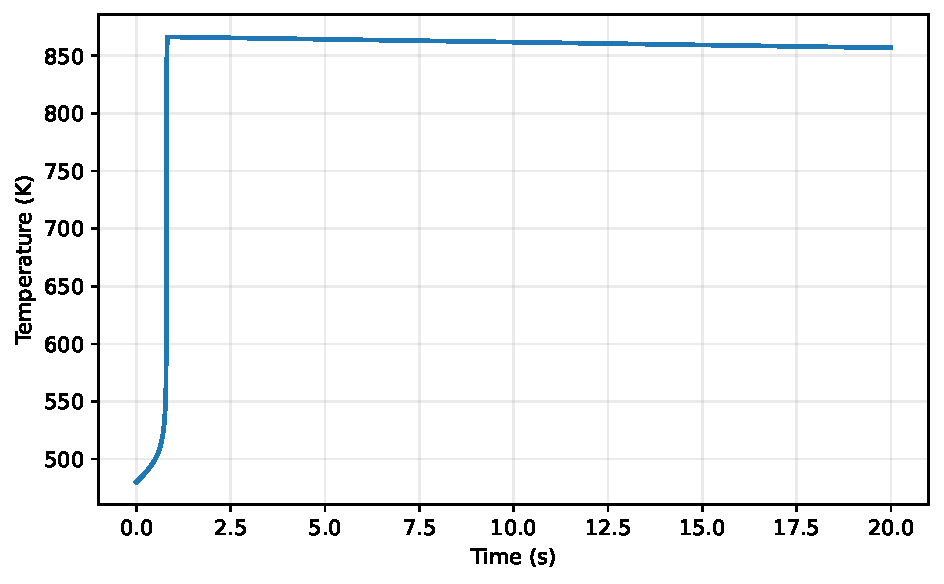
\includegraphics[
        width=0.78\textwidth
    ]{hu2020_temperature.pdf}

    \caption{
        Cell temperature predicted by LiionTR for the Hu et al.\
        reference thermal runaway simulation.
    }
    \label{fig:hu_temperature_result}
\end{figure}


\subsection{Reaction progression}

The evolution of the four reaction conversions is shown in
\cref{fig:hu_conversion_result}.

\begin{figure}[htbp]
    \centering
    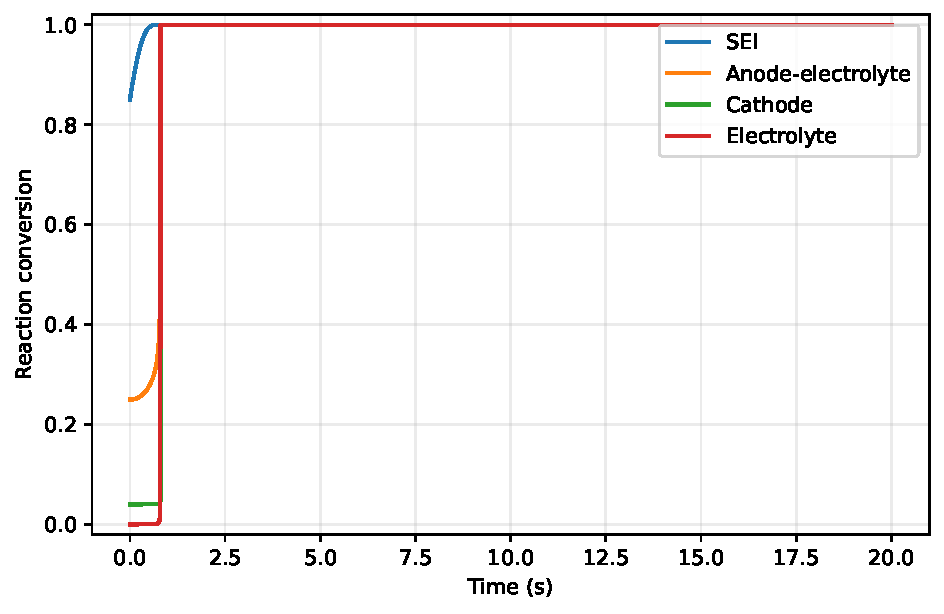
\includegraphics[
        width=0.82\textwidth
    ]{hu2020_conversion.pdf}

    \caption{
        Evolution of the SEI, anode-electrolyte, cathode, and electrolyte
        reaction conversions during the reference simulation.
    }
    \label{fig:hu_conversion_result}
\end{figure}


\subsection{Reaction heat generation}

The individual reaction contributions to heat generation are shown in
\cref{fig:hu_heat_result}.

\begin{figure}[htbp]
    \centering
    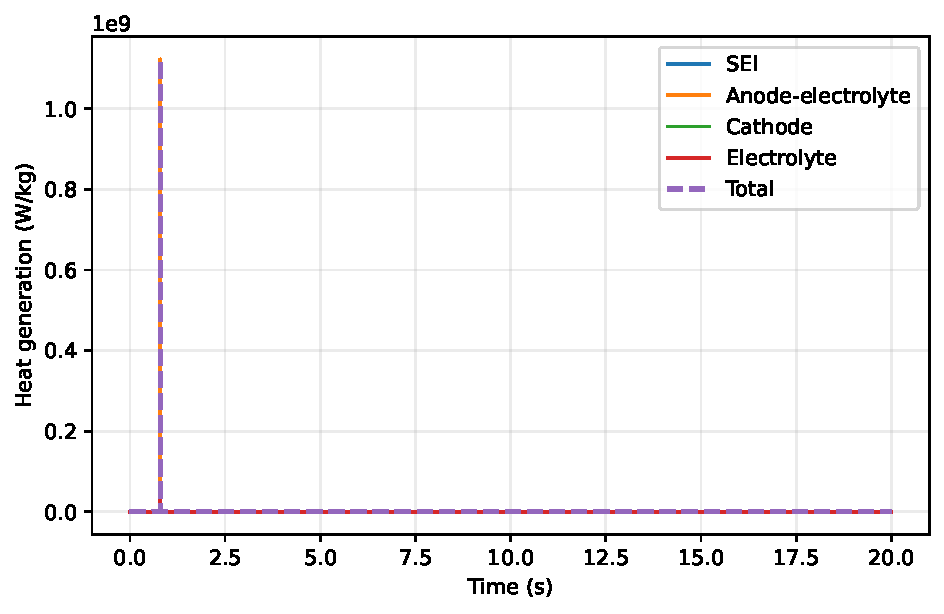
\includegraphics[
        width=0.82\textwidth
    ]{hu2020_heat_generation.pdf}

    \caption{
        Mass-specific heat-generation rates associated with the thermal
        runaway reactions in the Hu et al.\ reference simulation.
    }
    \label{fig:hu_heat_result}
\end{figure}

\subsection{Reaction-wise energy release}

Integration of the individual heat-generation rates provides the
specific energy released by each reaction during the reference
simulation.

The resulting energy balance is summarized in
\cref{tab:hu_reaction_summary}.

\input{generated/hu2020_reaction_summary}

\subsection{Energy distribution}

The energy distribution in
\cref{tab:hu_reaction_summary}
shows that the anode--electrolyte reaction is the dominant energetic
contribution in the present reference simulation.

It releases approximately

\begin{equation}
    q_{\mathrm{an}}
    =
    \SI{\HuAnodeEnergy}{\kilo\joule\per\kilogram},
\end{equation}

corresponding to approximately

\begin{equation}
    \HuAnodeFraction\%
\end{equation}

of the total reaction energy.

The cathode decomposition represents the second-largest contribution,

\begin{equation}
    q_{\mathrm{cat}}
    =
    \SI{\HuCathodeEnergy}{\kilo\joule\per\kilogram},
\end{equation}

or approximately

\begin{equation}
    \HuCathodeFraction\%
\end{equation}

of the total.

The electrolyte decomposition contributes

\begin{equation}
    q_{\mathrm{el}}
    =
    \SI{\HuElectrolyteEnergy}{\kilo\joule\per\kilogram},
\end{equation}

while SEI decomposition contributes only

\begin{equation}
    q_{\mathrm{SEI}}
    =
    \SI{\HuSeiEnergy}{\kilo\joule\per\kilogram}.
\end{equation}

The relatively small integrated SEI contribution is partly explained
by its initial reaction state. The SEI conversion is initialized at

\begin{equation}
    \alpha_{\mathrm{SEI},0}
    =
    0.85,
\end{equation}

so only a relatively small remaining fraction is available for further
decomposition during the simulated interval.

In contrast, the anode--electrolyte reaction begins at

\begin{equation}
    \alpha_{\mathrm{an},0}
    =
    0.25,
\end{equation}

leaving a substantially larger available reaction extent together with
a high specific reaction enthalpy.


\subsection{Reaction completion}

All four reaction states approach complete conversion during the
reference simulation,

\begin{equation}
    \alpha_i
    \rightarrow
    1.
\end{equation}

Consequently, the differences in integrated energy release are governed
primarily by the available reaction extent, reacting-material content,
reaction enthalpy, and, for the cathode, the relative contributions of
the two kinetic channels.

The cathode reaction deserves particular attention because its two
parallel kinetic channels share one conversion variable. Its integrated
energy therefore depends on the temperature-dependent partitioning of
reaction progress between the two channels and cannot generally be
represented by a single constant reaction enthalpy.


\subsection{Thermal response}

The combined reaction network releases

\begin{equation}
    q_{\mathrm{reaction}}
    =
    \SI{\HuIntegratedEnergy}{\kilo\joule\per\kilogram}
\end{equation}

during the simulated interval.

This heat release increases the lumped cell temperature from

\begin{equation}
    T_0
    =
    \SI{480}{\kelvin}
\end{equation}

to

\begin{equation}
    T_f
    =
    \SI{\HuFinalTemperature}{\kelvin}.
\end{equation}

The temperature evolution in
\cref{fig:hu_temperature_result}
reflects the positive feedback between Arrhenius reaction kinetics and
thermal energy release: increasing temperature accelerates the
exothermic reactions, which in turn generates additional heat.

The result should be interpreted as the response of the implemented
reduced-order model under the selected initial and boundary conditions,
rather than as a universal thermal runaway temperature for lithium-ion
cells.

The instantaneous thermal-power balance is shown in
\cref{fig:hu_thermal_power_balance}.

\begin{figure}[htbp]
    \centering
    \includegraphics[
        width=0.82\textwidth
    ]{hu2020_thermal_power_balance.pdf}

    \caption{
        Instantaneous mass-specific thermal-power balance for the
        Hu et al.\ reference simulation. Reaction heat generation is
        partitioned between sensible heating of the cell and convective
        heat transfer to the surroundings.
    }
    \label{fig:hu_thermal_power_balance}
\end{figure}

\subsection{Integrated reaction energy}

The total specific reaction energy is calculated from

\begin{equation}
    q_{\mathrm{reaction}}
    =
    \int
    \dot{q}_{\mathrm{total}}
    \,dt.
    \label{eq:results_integrated_heat}
\end{equation}

For the present reference calculation, the integrated reaction energy is
approximately

\begin{equation}
    q_{\mathrm{reaction}}
    =
    \SI{\HuIntegratedEnergy}{\kilo\joule\per\kilogram}.
\end{equation}

The final simulated cell temperature is approximately

\begin{equation}
    T_f
    =
    \SI{\HuFinalTemperature}{\kelvin}.
\end{equation}

These values characterize the selected numerical reference case and
should not be interpreted as general thermal runaway characteristics of
lithium-ion cells.

\section{Future Development}
\label{sec:future-work}
LiionTR is currently a reduced-order thermal runaway framework with
explicit models for reaction kinetics, heat generation, gas generation,
pressure, and venting.

Several extensions are required before the framework can represent the
full range of physical processes relevant to lithium-ion battery failure.

Development priorities are described below.


\subsection{Thermochemical gas modeling}

The current gas-generation formulation uses prescribed species yields.

This approach is useful for empirical models and verification but cannot
predict gas composition from the chemical state of the reacting battery
materials.

A future thermochemical formulation will represent reaction products in
terms of elemental inventories.

Conceptually,

\begin{equation}
    \text{thermal decomposition}
    \rightarrow
    \text{element source terms}
    \rightarrow
    \text{element inventory}
    \rightarrow
    \text{thermochemical equilibrium}.
\end{equation}

Relevant elements may include

\begin{equation}
    \mathrm{
        C,\,
        H,\,
        O,\,
        N,\,
        F,\,
        P,\,
        Li
    }.
\end{equation}

A thermochemical equilibrium backend can then determine gas composition
subject to specified thermodynamic constraints.


\subsection{Cantera integration}

Cantera is a strong candidate for the thermochemical backend.

A future LiionTR interface may provide a generic abstraction such as

\begin{equation}
    \texttt{GasEquilibriumBackend},
\end{equation}

with a Cantera implementation responsible for

\begin{itemize}
    \item equilibrium gas composition;
    \item mixture molar mass;
    \item heat capacities;
    \item enthalpy and internal energy;
    \item heat-capacity ratio;
    \item other thermodynamic properties required by venting.
\end{itemize}

The initial implementation may use constant-volume, constant-temperature
equilibrium calculations.

More advanced formulations may require coupled energy-conserving
equilibrium calculations.


\subsection{Energy-consistent thermochemistry}

The current thermal state is temperature.

This is convenient for reduced-order calculations but may become
insufficient when significant energy is redistributed through chemical
equilibrium, vaporization, gas discharge, or phase change.

A future formulation may therefore evolve internal energy,

\begin{equation}
    U,
\end{equation}

rather than temperature directly.

Temperature would then be reconstructed from the thermodynamic state,

\begin{equation}
    T
    =
    T
    \left(
        U,
        V,
        \mathbf{n}
    \right).
\end{equation}

Such a formulation would provide a more rigorous basis for energetic
coupling between condensed reactions and gas-phase thermochemistry.


\subsection{Electrochemical coupling}

Thermal runaway behavior depends strongly on the electrochemical state
of the cell.

Relevant quantities include

\begin{itemize}
    \item state of charge;
    \item electrode lithium concentration;
    \item electrode potential;
    \item current;
    \item irreversible electrochemical heating;
    \item reversible entropic heating.
\end{itemize}

PyBaMM may eventually provide these quantities to LiionTR.

The intended coupling is not to replace PyBaMM electrochemistry, but to
allow electrochemical state variables to modify thermal runaway kinetics,
reaction inventories, or onset conditions.


\subsection{Calorimetric parameter estimation}

Thermal runaway kinetic parameters are often derived from differential
scanning calorimetry or accelerating rate calorimetry measurements.

LiionTR may therefore include tools for fitting model parameters to
experimental data.

Potential parameters include

\begin{equation}
    A,
    \qquad
    E_a,
    \qquad
    \Delta H,
    \qquad
    n,
    \qquad
    \alpha_0.
\end{equation}

Parameter estimation could be formulated as an optimization problem,

\begin{equation}
    \boldsymbol{\theta}^{*}
    =
    \arg\min_{\boldsymbol{\theta}}
    J
    \left(
        \boldsymbol{\theta}
    \right),
\end{equation}

where $\boldsymbol{\theta}$ is the parameter vector and $J$ measures the
difference between simulation and experiment.


\subsection{Sensitivity and uncertainty analysis}

Published thermal runaway parameters can vary substantially between
cells, chemistries, measurement methods, and states of charge.

Future development should therefore consider parameter uncertainty.

Relevant outputs may include sensitivities of

\begin{itemize}
    \item thermal runaway onset time;
    \item maximum temperature;
    \item maximum pressure;
    \item vent-opening time;
    \item total gas generation;
    \item total energy release.
\end{itemize}

Both local sensitivity analysis and Monte Carlo uncertainty propagation
may be useful.


\subsection{Temperature-dependent material properties}

The current cell thermal properties are effectively constant.

Future material models may support

\begin{equation}
    c_p
    =
    c_p(T),
\end{equation}

\begin{equation}
    k
    =
    k(T),
\end{equation}

and potentially

\begin{equation}
    \rho
    =
    \rho(T).
\end{equation}

Phase transitions and latent-heat effects may also be relevant at severe
thermal runaway temperatures.


\subsection{Spatial thermal models}

The present lumped formulation cannot reproduce internal temperature
gradients.

A natural extension is a one-dimensional radial model for cylindrical
cells,

\begin{equation}
    \rho c_p
    \frac{\partial T}{\partial t}
    =
    \frac{1}{r}
    \frac{\partial}{\partial r}
    \left(
        k r
        \frac{\partial T}{\partial r}
    \right)
    +
    \dot{q}_{\mathrm{gen}}.
\end{equation}

More general finite-volume or finite-element formulations could later
support cylindrical, prismatic, and pouch cells.


\subsection{Cell-to-cell propagation}

Battery-module safety analysis requires coupling between multiple cells.

For cell $i$, a generic thermal balance may be written as

\begin{equation}
    C_i
    \frac{dT_i}{dt}
    =
    \dot{Q}_{i,\mathrm{gen}}
    -
    \dot{Q}_{i,\mathrm{ambient}}
    +
    \sum_j
    \dot{Q}_{j\rightarrow i}.
\end{equation}

The inter-cell term

\begin{equation}
    \dot{Q}_{j\rightarrow i}
\end{equation}

may include conduction, radiation, convection, or heat transfer from
vent gases and flames.

The modular cell representation already provides a basis for this
extension.


\subsection{Mechanical venting and rupture}

The current vent-opening model uses a prescribed pressure threshold and
instantaneous transition to a fixed vent area.

More realistic models may include

\begin{itemize}
    \item progressive vent displacement;
    \item pressure-dependent vent area;
    \item burst-disk failure;
    \item casing deformation;
    \item rupture;
    \item multiple vent paths.
\end{itemize}

A mechanical model could therefore determine

\begin{equation}
    A_v
    =
    A_v
    \left(
        P,
        T,
        t
    \right)
\end{equation}

instead of treating vent area as constant.


\subsection{Multiphase venting}

Real battery vent products may contain gases, vapor, droplets, aerosols,
and solid particles.

The current single-phase ideal-gas discharge model does not represent
these phenomena.

Future formulations may require

\begin{itemize}
    \item electrolyte vaporization;
    \item flashing flow;
    \item liquid entrainment;
    \item aerosol transport;
    \item multiphase choking criteria.
\end{itemize}


\subsection{External vent-jet and combustion models}

Once material leaves the cell, additional physical processes may occur
outside the battery.

These include

\begin{itemize}
    \item turbulent jet formation;
    \item mixing with ambient air;
    \item ignition;
    \item flame propagation;
    \item radiant heat transfer;
    \item toxic-species transport.
\end{itemize}

These processes are outside the current LiionTR domain but could
eventually be represented through interfaces to combustion or
computational-fluid-dynamics tools.


\subsection{Validation database}

A robust thermal runaway framework requires systematic comparison with
experimental measurements.

A future validation database could contain

\begin{itemize}
    \item battery-cell metadata;
    \item chemistry;
    \item geometry;
    \item nominal capacity;
    \item state of charge;
    \item abuse condition;
    \item ARC data;
    \item DSC data;
    \item temperature histories;
    \item pressure histories;
    \item vent gas composition;
    \item vented mass;
    \item photographs or high-speed imaging metadata.
\end{itemize}

Standardized datasets would permit repeatable comparison between
alternative LiionTR models.


\subsection{Software development}

In addition to physical-model development, several software improvements
are anticipated:

\begin{itemize}
    \item stable public APIs;
    \item structured serialization of simulations;
    \item model configuration files;
    \item reproducible simulation metadata;
    \item plotting and post-processing utilities;
    \item parameter databases;
    \item expanded example simulations;
    \item automated benchmarking;
    \item optional parallel parameter studies.
\end{itemize}


\subsection{Long-term architecture}

The long-term architecture can be summarized conceptually as

\begin{equation}
    \boxed{
    \begin{array}{c}
        \text{Electrochemistry} \\
        \text{PyBaMM}
    \end{array}
    }
    \longrightarrow
    \boxed{
    \begin{array}{c}
        \text{Thermal runaway} \\
        \text{LiionTR}
    \end{array}
    }
    \longrightarrow
    \boxed{
    \begin{array}{c}
        \text{Thermochemistry} \\
        \text{Cantera}
    \end{array}
    }.
\end{equation}

LiionTR is intended to remain the layer responsible for coordinating
battery-safety-specific physics, thermal runaway reactions, gas
generation, pressure, venting, and propagation.

The framework should therefore remain modular enough that increasing the
fidelity of one physical subsystem does not require redesigning the
complete simulation architecture.

\newpage

\printbibliography

\end{document}